%!TEX root = ../dissertation.tex
\chapter{Validation Studies}
\label{chap:experiments}
In this section, verification and validation of various aspects of the numerical method discussed in Section \S\ref{chap:discrete_Model} and \S\ref{chap:continua_Model} are presented. Specifically, the numerical method discussed in Section \S\ref{sec:ISPH}  is compared with a finite element counterpart in Section \S\ref{sec:Eu_La}. Comparison of numerical methods presented in Sections \S\ref{sec:WCSPH}, \S\ref{sec:ISPH}, and \S\ref{sec:KCSPH} is described in Section \S\ref{sec:Lag_Lag}. Verification and validation of the IISPH method (\S\ref{sec:IISPH}) is described in Section \S\ref{sec:IISPH_Val}. Lastly, the use of regularization (\S\ref{sec:Uniqueness}) for obtaining a unique solution for the DVI method is studied in Section \S\ref{sec:DVI_Uniq}. 



\section{Lagrangian vs. Eulerian Discretization of Continua}\label{sec:Eu_La}
We report the results of a study in which we compared the Eulerian and Lagrangian approaches for the solution of free-surface and Fluid-Solid Interaction (FSI) problems. The Eulerian approach is implemented in another open-source code -- Proteus \cite{proteus_1_6_1}, which embraces the Finite Element Method (FEM). Four tests were considered in this study: flow around a cylinder, dam break, falling yet floating cylinder in a fluid tank, and an elastic gate problem. We conclude that the SPH methodology is permissive and expeditious. When compared to a more robust Eulerian method such as FEM, the SPH solver produces a solution that is reasonably accurate, computationally less demanding, and easier to produce for the class of problems investigated in this work.  The FEM solver is more accurate as are the methods it draws on.


\subsection{The Eulerian Model}\label{sec:Eulerian}
In the Eulerian approach, we consider two incompressible Newtonian phases, air and water, separated by a sharp material interface, across which density and viscosity are discontinuous, but velocity and pressure are continuous. Surface tension is, therefore, neglected. 

Denote the domains of the air and water phases as 
$\Omega_a(t)$ and $\Omega_w(t)$. The whole domain is $\Omega = \Omega_w(t)\cup\Omega_a(t)$ and the air/water interface is $\Gamma(t) = \overline{\partial\Omega_w(t)}\cap \overline{\partial\Omega_a(t)}$. 
The Navier-Stokes equation above is used to model the motion of each phase of fluid
\begin{align}
\begin{cases}
\rho_i\frac{\partial \vect{u}_i}{\partial t} + \rho_i \vect{u}_i\cdot\nabla\vect{u}_i = -\nabla p_i + \nabla\cdot \bm{\tau}_i+\vect{f}_i,\quad \vect{x}\in\Omega_i(t)\\
\nabla\cdot\vect{u}_i = 0 \; 
\end{cases},\label{eq:Eulerian_NS}
\end{align}
where $\vect{u}_i$ is the velocity, $p_i$ is the pressure, $\vect{f}$ is the body force, 
$\mu_i$ is the dynamic viscosity, $\bm{\sigma}_i \equiv -p_i\bI+ 2\mu\bm{\epsilon}(\vect{u}_i)$ is the stress tensor, 
$\bm{\epsilon}(\vect{u})\equiv \frac{1}{2}(\nabla\vect{u}+\nabla\vect{u}^T)$, 
and $i\in \{w,a\}$. 

To solve the Navier-Stokes equations, Eq.~\ref{eq:Eulerian_NS}, 
one has to provide proper boundary conditions on the exterior boundary $\partial\Omega$ and on the interface 
$\Gamma(t)$. The boundary condition on $\partial\Omega$
depends on the problem, and, based on the assumption of continuity of velocity and stress across the interface, 
\begin{align}
\label{eq:interface_condition}
p_a = p_w, \quad \vect{u}_a = \vect{u}_w, \quad {\vect\sigma}_a \cdot \vect{n} = {\vect\sigma}_w \cdot \vect{n},\quad \vect{x}\in\Gamma(t) \; .
\end{align}
Using this interface condition (Eq.~\ref{eq:interface_condition}) and neglecting the potential loss of smoothness due to the jump discontinuities in density and viscosity, we can introduce continuous global pressure and velocity fields $p$ and $\vect{u}$ and solve a single Navier-Stokes equation
\begin{align*}
\begin{cases}
\rho\frac{\partial \vect{u}}{\partial t} + \rho\vect{u}\cdot\nabla\vect{u} = -\nabla p + \nabla\cdot (2\mu\bm{\epsilon}(\bm u))+\vect{f},\quad \vect{x}\in\Omega\\
\nabla\cdot\vect{u} = 0 
\end{cases},
\end{align*}
in the whole domain $\Omega$, with $\rho := \rho_w 1_{x\in\Omega_w(t)}+\rho_a 1_{x\in\Omega_a(t)}$ and 
$\mu := \mu_w 1_{x\in\Omega_w(t)}+\mu_a 1_{x\in\Omega_a(t)}$. Note that $\rho$ and $\mu$ vary in time and space due the dynamic interface $\Gamma(t)$. In this work we use a conservative level set scheme described in \cite{KAFB11}, which represents the interface $\Gamma(t)$ implicitly as the zero level set
\begin{equation}
\phi(t,\vect{x}) = 0 \; ,
\end{equation}
where $\phi$ is the negative of the signed distance to $\Gamma(t)$ within the water phase and the positive signed distance in the air phase.

In this approach both an air volume fraction, $\theta$, and the dynamics of the signed distance field, $\phi$, are modeled based on the governing equations for material surface motion
\begin{align}
\label{eq:ls_transport_1}
\frac{\partial \phi}{\partial t} + \vect{u}\cdot\nabla\phi = 0 \; ,
\end{align}
and phase volume conservation
\begin{align}
\label{eq:ls_transport_2}
\frac{\partial \theta}{\partial t} + \nabla\cdot(\vect{u}\theta) = 0 \; .
\end{align}
We then compute $\rho$ and $\mu$ as 
\begin{align}
\label{eq:two_phase_rho}
\rho(t,\vect{x}) = \rho_w [1-H(\phi)] + \rho_a H(\phi),\\
\label{eq:two_phase_nu}
\mu(t,\vect{x}) = \mu_w [1-H(\phi)] + \mu_a H(\phi) \; ,
\end{align}
where $H(\cdot)$ is the Heaviside step function. 

As the solution evolves, the level set $\phi$ will gradually lose the signed distance property and the phase mass conservation property. To simplify the presentation, we assume that there is no flow through external boundaries, so that for all time the air mass $M_a$ should maintain the phase mass conservation property
\begin{equation}
M_a = \int_{\Omega} \rho_a H(\phi(t,\vect{x}) \; .
\end{equation}
Note that, under the given assumptions, this statement can be written equivalently as a volume conservation statement and that analogous statements hold for the water phase.

Several methods have been proposed to correct the violation of these conservation constraints, see, for instance~\cite{Sussman2000,PSVW2004}. 
Here we are correcting $\phi$ based on the conserved quantity $\theta$ as suggested in~\cite{KAFB11}. The idea is to compute the correction $u$ satisfying the equation
\begin{align}
\label{eq:mass_correction}
H(\phi+u) - \theta = \nu_{num} \Delta u,
\end{align}
in order to keep the mass conservation.

As noted above, the use of continuous and differentiable fields for pressure and velocity over the entire domain $\Omega$ is an approximation that is inconsistent with actual jump discontinuities in density and viscosity. In fact, we use a regularized Heaviside function, $H_\epsilon(x)$ as follows
\begin{align}
\label{eq:approx_H}
H_{\epsilon}(x) := \begin{cases}
0, \quad \text{ if }x\leq -\epsilon\\
\frac{1}{2}(1+\frac{x}{\epsilon}+\frac{1}{\phi_{ls}}\sin(x\frac{\phi_{ls}}{\epsilon}))\quad\text{ if }|x|\leq \epsilon\\
1, \quad \text{ if }x\geq \epsilon
\end{cases} \; ,
\end{align}
to approximate $H(x)$ used in Eqs.~\ref{eq:two_phase_rho} and~\ref{eq:two_phase_nu}. This represents a first order regularization of the two-phase flow problem. While much prior work uses this regularization, notable recent research provides methods and proofs that more precise, second order accurate treatment of the fluid-fluid interface is achievable in the finite element context \cite{burman2015cutfem,ji2016ifem}.

The practice of reinitializing the level set function is a well-established technique in two-phase flow to control the growth of anomalies and/or numerical errors \cite{trujillo2017distortion}. In the present work, we correct the loss of the signed distance property by solving
\begin{align}
\label{eq:reinitialization}
\partial_\tau \phi + \text{sign}(\phi)(|\nabla\phi|-1) = 0 \; ,
\end{align}
subject to boundary conditions $\phi=0$ on $\Gamma(t)$ (i.e., the distance correction does not move the air-water interface).

The algorithm for the time step $t^n \rightarrow t^{n+1}$ can be described as follows:
\begin{enumerate}
	\item Solve Eq.~\ref{eq:Eulerian_NS} with $\rho(t^n)$ and $\mu(t^n)$ defined in Eqs.~\ref{eq:two_phase_rho} and~\ref{eq:two_phase_nu} to get the velocity field $\vect{u}^{n+1}$ and pressure $p^{n+1}$ \label{listItem:uANDp}
	\item Solve Eq.~\ref{eq:ls_transport_1} to get $\phi^*(t^{n+1})$
	\item Solve Eq.~\ref{eq:ls_transport_2} to get $\theta^*(t^{n+1})$
	\item Solve Eq.~\ref{eq:reinitialization} to get $\phi^{**}(t^{n+1})$ from $\phi^*(t^{n+1})$
	\item Solve~\ref{eq:mass_correction} to get corrected $\phi(t^{n+1})$ and $\theta=H_{\epsilon}(\phi)$ using $\phi^{**}(t^{n+1})$ and $\theta^*(t^{n+1})$.
\end{enumerate}

We use continuous finite elements to implement an IBM for the solid phase boundary as well.
Let $V_h$ and $M_h$ be the approximation space of the velocity and the pressure. For the incompressible Navier-Stokes equations, not all pairs $V_h\times M_h$ of piecewise polynomial spaces are stable, see, for instance~\cite{Arnold1990, EG04}. In addition to instabilities that can arise due to the choice of velocity and pressure spaces, the numerical solution of the Navier-Stokes equations for $Re>1$ can also experience advective instabilities, resulting in velocity (and pressure) oscillations. In this work we follow the variational multiscale stabilization and shock capturing method used previously in \cite{KAFB11}, which introduces additional numerical viscosity in a manner that stabilizes the advective instabilities as well as the equal-order velocity and pressure spaces. As these additional terms are unchanged from \cite{KAFB11}, we will simply reference them as $(stabilization-terms)$ below. Thus, in addressing point \ref{listItem:uANDp} above, the numerical method used produces $\vect{u}^{n+1}\in V_h$ and $p^{n+1}\in M_h$ such that 
\begin{align}
&\int_\Omega\rho \frac{\vect{u}^{n+1}-\vect{u}^n}{\tau}\cdot\vect{v} - (\rho \vect{u}^{n+1}\cdot \nabla \vect{u}^{n+1})\cdot \vect{v} 
+\nabla p^{n+1}\cdot\vect{v} +2\mu\varepsilon(\vect{u}^{n+1}):\varepsilon(\vect{v})
-\vect{f}\cdot\vect{v}\nonumber\\
&+\int_\Omega [-2\mu \varepsilon(\vect{u}^{n+1})\vect{n}\cdot\vect{v}
-2\mu\varepsilon(\vect{v})\vect{n}\cdot(\vect{u}^{n+1}-\vect{u}_S^{n+1})
+C_\alpha\vect{v}\cdot(\vect{u}^{n+1}-\vect{u}_S^{n+1})]\delta_\epsilon(d_{\partial\Omega_S(t^{n+1})}(\vect{x}))\nonumber\\
&+\int_\Omega C_\beta (\vect{u}^{n+1}-\vect{u}_S^{n+1})\cdot\vect{v} H_\epsilon(d_{\partial\Omega_S(t^{n+1})}(\vect{x}))\nonumber\\
&+\int_\Omega \vect{u}^{n+1}\cdot\nabla q \nonumber\\
&+\int_{\partial\Omega_D} [-2\mu\varepsilon(\vect{u}^{n+1})\vect{n}\cdot\vect{v}
-2\mu\varepsilon(\vect{v})\vect{n}\cdot(\vect{u}^{n+1}-\vect{u}_D^{n+1})
+C_\gamma\vect{v}\cdot(\vect{u}^{n+1}-\vect{u}_D^{n+1})]\nonumber\\
&+(stabilization-terms)=0 \quad\forall \vect{v}\in V_h, q\in M_h \; ,
\end{align}
where $\varepsilon(\vect{u}) = (\nabla \vect{u} + \nabla \vect{u}^2)$ and $C_{\alpha}$, $C_{\beta}$, and $C_{\gamma}$ are numerical parameters. In this formulation, the first row is the weak formulation of Navier-Stokes equations with integration-by-parts applied to the  viscous term; the second row is the Nitsche's method for enforcing the no-slip boundary
condition on the surface of the solid, using the regularized Dirac delta function $\delta_{\epsilon}$ (derived from Eq.~\ref{eq:approx_H}) to replace the boundary integral with a volume integral; the third row is the penalty term on the velocity inside 
the solid; the fourth row is from the continuity equation; the fifth row is due to the boundary condition of $\vect{u}|_{\partial\Omega_D}(t)=\vect{u}_D(t)$ and $2\nu\epsilon(\vect{u})\cdot\vect{n}|_{\partial\Omega_N}(t)=\vect{g}(t)$ with $\partial\Omega_D\cap\partial\Omega_N=\emptyset$ and  $\partial\Omega=\partial\Omega_D\cup\partial\Omega_N$.

We solve this system using a first-order operating splitting scheme for variable-coefficient Navier-Stokes equations following \cite{GS09}. The first step is to solve for the velocity $\tilde{\vect{u}}^{n+1}$ by solving
\begin{align}
&\int_\Omega\rho\frac{\tilde{\vect{u}}^{n+1}-\vect{u}^n}{\tau}\cdot\vect{v} + \rho(\vect{u}^*\cdot\nabla\tilde{\vect{u}}^{n+1}) \cdot \vect{v} 
+\nabla p^{\#}\cdot\vect{v} +2\mu \varepsilon(\tilde{\vect{u}}^{n+1}):\varepsilon(\vect{v})
-\vect{f}\cdot\vect{v}\nonumber\\
&+\int_\Omega [-2\mu \varepsilon(\tilde{\vect{u}}^{n+1})\vect{n}\cdot\vect{v}
-2\mu\varepsilon(\vect{v})\vect{n}\cdot(\tilde{\vect{u}}^{n+1}-\vect{u}_S^{n+1})
+C_\alpha\vect{v}\cdot(\tilde{\vect{u}}^{n+1}-\vect{u}_S^{n+1})]\delta_\epsilon(d_{\partial\Omega_S(t^{n+1})}(\vect{x}))\nonumber\\
&+\int_\Omega C_\beta (\tilde{\vect{u}}^{n+1}-\vect{u}_S^{n+1})\cdot\vect{v} H_\epsilon(d_{\partial\Omega_S(t^{n+1})}(\vect{x}))\nonumber\\
&+\int_{\partial\Omega_D} [-2\mu\varepsilon(\vect{u}^{n+1})\vect{n}\cdot\vect{v}
-2\mu\varepsilon(\vect{v})\vect{n}\cdot(\vect{u}^{n+1}-\vect{u}_D^{n+1})
+C_\gamma\vect{v}\cdot(\vect{u}^{n+1}-\vect{u}_D^{n+1})]-\int_{\partial\Omega_N}\vect{g}\cdot\vect{v}\nonumber\\
&+(stabilization-terms)=0,\quad\forall \vect{v}\in V_h \; ,
\end{align}
where $\vect{u}^*$ and $p^\#$ are the extrapolation of the velocity and the pressure computed as $\vect{u}^*:=\vect{u}^n$ and $p^\#:=p^n+\phi^{n}$. This choice results in a linear system for the velocity components.
The 2nd step of the projection scheme corrects the velocity field $\tilde{\vect{u}}^{n+1}$ to obtain 
a divergence free velocity field ${\vect{u}}^{n+1}$ and an accurate pressure, $p^{n+1}$. The velocity field $\tilde{\vect{u}}^{n+1}$ is defined as 
\begin{align*}
\tilde{\vect{u}}^{n+1} = \tilde{\vect{u}}^{n+1} - \frac{\tau}{\rho_{\min}}\nabla\phi^{n+1} \; ,
\end{align*}
with the help of the pressure increment, $\phi^{n+1}$, which satisfies the Poisson problem 
\begin{align*}
\nabla\cdot\nabla\phi^{n+1} = \nabla\cdot\tilde{\vect{u}}^{n+1} ,
\end{align*}
with appropriate boundary conditions. For example, at the part of the boundary where $\vect{u}^{n+1}$ and 
$\tilde{\vect{u}}^{n+1}$ are specified, one has to enforce $\nabla\phi^{n+1}\cdot\vect{n}=0$.
The pressure $p^{n+1}$ is then defined as 
\begin{align*}
p^{n+1} := p^n + \phi^{n+1} - \mu \nabla\cdot\tilde{\vect{u}}^{n+1} \; .
\end{align*}
Details pertaining the stability of this algorithm and a proof of second order accuracy in time when a second order BDF method is used in place of Backward
Euler used above are provided in~\cite{GS09}. 

In the following, we present and discuss results obtained with the Eulerian and Lagrangian approaches for four tests. The flow around a cylinder is considered, given that it represents a widely used single-phase CFD benchmark problem. A dam break test is used to gauge performance for free-surface flows. Lastly, the two approaches are compared in conjunction with two FSI problems -- one pertaining to a floating rigid body and one that has the fluid interacting with an elastic/deformable gate. 

\subsection{Flow Around Cylinder}
\label{subsec:flowAroundCylinder_fsi}
This single-phase, internal flow test is used to compare the FE and SPH solutions for a benchmark problem where the flow is shaped by the interplay between the pressure gradient, and the viscous and body forces. The cylinder of radius 0.05\si{m} is positioned at the center of a rectangular domain of height 0.4\si{m} and length 1.0\si{m}. No-slip boundary conditions are applied to the top and bottom walls while periodic (cyclic) conditions are maintained at the left (inlet) and right (outlet) patches. A constant body force $\mathbf{f}_b$=1.0\si{m/s^2} is applied in order to balance the viscous force. The density and viscosity are set to $\rho_0$=10.0\si{kg/m^3} and $\mu$=0.1\si{Pa.s}, respectively. As illustrates in Fig~\ref{fig:FoCV_fsi}, the steady-state {\textit{velocity}} predicted by SPH and FEM are qualitatively in close agreement.
\begin{figure}[H]
	\centering    
	\begin{subfigure}{0.45\columnwidth}    
		\centering
		\includegraphics[width=1.0\textwidth]{images/FSI_Comparison/FOC_U.png}
	\end{subfigure}
	
	\begin{subfigure}{0.47\columnwidth}    
		\centering
		\includegraphics[width=1.0\textwidth]{images/FSI_Comparison/FOC_SPH_U.png}
	\end{subfigure}
	\begin{subfigure}{0.47\columnwidth}
		\centering
		\includegraphics[width=1.0\textwidth]{images/FSI_Comparison/FOC_FEM_U.png}
	\end{subfigure}
	\caption{Comparison of the steady-state velocity profiles predicted with SPH (left) and FEM (right). The SPH markers outside the fluid domain are BCE markers, see \S\ref{sec:BC}.}    \label{fig:FoCV_fsi}
\end{figure} 
% Obtaining the correct smooth pressure field in SPH is generally a more challenging task than in FEM. In Weakly Compressible types of SPH, this is manifested in severe checker-boarding patterns in the pressure field, which happens due to the use of a stiff equation of state for pressure as well as the decoupling of pressure and velocity fields. Historically, the checker-boarding artifact has been fixed in Eulerian methods such as FD method by using \textit{staggered} grids. In staggered grids, the scalar field variables are stored in cell centers while the velocities are stored at the cell faces. This artifact is overcome in FV method by Rhie-Chow type of methods which make it possible to use \textit{collocated} grids as opposed to staggered ones. FE overcomes this artifact by requiring a mixed FE space seen in the Taylor\-Hood elements, in which lower-order approximation space is used for pressure comparing to velocity.  Our implicit SPH formulation although is more robust than WCSPH in terms of handling the checker-boarding effects, still may show this artifact in highly transient problems where the density of individual particles drops below the rest density. In such cases, the free-surface boundary condition for pressure ($p=0$) kicks in and causes a zigzaggy pressure field in the neighborhood of the particles with low density.
Similarly, the FEM and SPH pressure profiles show close agreement as illustrated in Fig.~\ref{fig:FoCP_fsi}.
\begin{figure}[H]
	\centering
	\begin{subfigure}{0.45\columnwidth}    
		\centering
		\includegraphics[width=1.0\textwidth]{images/FSI_Comparison/FOC_p.png}
	\end{subfigure}
	
	\begin{subfigure}{0.47\columnwidth}    
		\centering
		\includegraphics[width=1.0\textwidth]{images/FSI_Comparison/FOC_SPH_p.png}
	\end{subfigure}
	\begin{subfigure}{0.47\columnwidth}
		\centering
		\includegraphics[width=1.0\textwidth]{images/FSI_Comparison/FOC_FEM_p.png}
	\end{subfigure}
	\caption{Comparison of the steady-state pressure profiles predicted with  SPH (left) and FEM (right). }    \label{fig:FoCP_fsi}
\end{figure} 
Lastly, we quantitatively compare the two methods in terms of drag calculation. Herein, the expression used for the drag coefficient is $C_d=\frac{F_d}{0.5\rho\;A\; U^2}$, where $F_d$ is the drag force magnitude along the $x$ axis, $\rho=\rho_0$ and $U=1$\si{m/s} are the reference density and velocity, and $A$ is the frontal area of the cylinder.  As shown in Fig.~\ref{fig:FoC_fsi}, SPH and FEM show different drag coefficients at the onset of the simulation yet the steady-state solutions are in good agreement-- the relative error of the time-averaged drag coefficient over the last 2\si{s} of the simulations is $6.4$\%. We posit that two reasons contributing to these discrepancies are: ($i$) the different time-integration schemes, and ($ii$) the vastly different space discretization technique and boundary condition enforcement used in the formulations. The IB method requires a fine mesh near the solid level-set (cylinder) for accurate representation of the fluid-structure interface and forces. Handling this interface poses no major challenge to SPH or boundary-fitted mesh-based approaches, owing to the explicit representation of the fluid-structure interface.
\begin{figure}[H]
	\begin{center}
		\vspace{-10pt}
		\includegraphics[width=0.5\textwidth]{images/FSI_Comparison/Figure_flow_around_cylinder.png}
	\end{center}
	\caption{Variation of the drag coefficient over time.}
	\label{fig:FoC_fsi}
	%    \vspace{-20pt}
\end{figure}

\subsection{Dam Break}
This free-surface flow experiment is setup as follows: the fluid domain is a rectangular prism of size 2\si{m} $\times$ 1.0\si{m}. The reference density and viscosity are $\rho=1000$\si{kg/m^3} and $\mu=$\SI{0.001}{Pa.s}. The gravity $g=-9.8$\si{m/s^2} is applied in the  $y$ direction. The SPH and FEM results are compared from two perspectives: $(i)$ the fluid front position over time, and $(ii)$ the roll up and the second splash -- two characteristics highlighted in previous studies \cite{colagrossi2003numerical,Adami2012}. As shown in Fig.~\ref{fig:db_front_fsi}, the SPH solution of the fluid front position over time slightly under-estimate the FEM solution. SPH has an easier task in handling free-surface since in the Lagrangian framework solving the Navier-Stokes equation (Eq.~\ref{eq:NS_IN_Lagrangian}) automatically provides for a tracking of the free-surface  \cite{Martin1952,colagrossi2003numerical,hughes2010comparison,xu2016improved,miladHalfImplicit2018}. In contrast, the Eulerian framework calls for four additional equations: ($i$) the advection of the level-set field via the velocity (Eq.~\ref{eq:ls_transport_1}); ($ii$) the conservation of the volume fraction (Eq.~\ref{eq:ls_transport_2}); ($iii$) level-set correction (re-initialization) (Eq.~\ref{eq:reinitialization}); and ($iv$) the mass correction (Eq.~\ref{eq:mass_correction}). While recent work \cite{quezadadeluna2019monolithic} demonstrates that this multistage algorithm can be collapsed into a single stage, it nevertheless represents significant added complexity in the implementation.
\begin{figure}[H]
	\begin{center}
		\includegraphics[width=0.5\textwidth]{images/FSI_Comparison/Figure_damBreak.png}
	\end{center}
	\caption{Comparison of water-front propagation between between SPH and FEM.}
	\label{fig:db_front_fsi}
\end{figure}
With regard to the roll-up and second splash characteristics, both methods predict well these two hallmark features of the dam break experiment, see Fig.~\ref{fig:db_charac_fsi}.
\begin{figure}[H]
	\centering    
	\begin{subfigure}{0.35\columnwidth}    
		\centering
		\includegraphics[width=1.0\textwidth]{images/FSI_Comparison/DB_U.png}
	\end{subfigure}
	
	\begin{subfigure}{0.4\columnwidth}    
		\centering
		\includegraphics[width=1.0\textwidth]{images/FSI_Comparison/DB_FEM_1.png}
	\end{subfigure}
	\begin{subfigure}{0.4\columnwidth}
		\centering
		\includegraphics[width=1.0\textwidth]{images/FSI_Comparison/DB_FEM_2.png}
	\end{subfigure}
	\begin{subfigure}{0.4\columnwidth}    
		\centering
		\includegraphics[width=1.0\textwidth]{images/FSI_Comparison/DB_SPH_1.png}
	\end{subfigure}
	\begin{subfigure}{0.4\columnwidth}
		\centering
		\includegraphics[width=1.0\textwidth]{images/FSI_Comparison/DB_SPH_2.png}
	\end{subfigure}
	\caption{Comparison of the roll-up ($t=1.75$\si{s}, left) and the second splash ($t=2.05$\si{s}, right) characteristics between FEM (top) and SPH (bottom)}    
	\label{fig:db_charac_fsi}
\end{figure}

\subsection{Fluid Interaction with a Falling Cylinder}
This experiment was used to compare the Eulerian and Lagrangian approaches in conjunction with a 3D scenario that included ample fluid-solid boundary movement. It may be regarded as a simplified problem that, in more complex forms, is conspicuous in several fluid-structure interaction applications in coastal and offshore structures, e.g., renewable energy devices and caissons. Insofar as the solution methodology is concerned, the test assesses the robustness of the fluid-structure coupling methodology described in
\S\ref{sec:FSI}. 

The problem is setup as follows. A cylindrical object of radius $r=0.12$\si{m} and length $L=0.2$\si{m} is released from the height $h=0.25$\si{m} above the surface of a tank of water at $t=0$\si{s}. The dimension of the fluid domain is 1.0\si{m} $\times$ 1.0\si{m} $\times$ 0.2\si{m} (width$\times$height$\times$depth). The gravity $g=-9.8$\si{m/s^2} is applied in the $y$ direction. The reference density and viscosity of the water are $\rho=1000$\si{kg/m^3} and $\mu=$\SI{0.001}{Pa.s}. The density of the cylinder is $\rho_s=0.7\rho$, which turns it into a floating structure. Figure~\ref{fig:CD} illustrates the distribution of the pressure in the frontal cross-section of the domain at $t=0.5$\si{s}. 

The cylinder oscillates until its initial potential energy is damped out. The steady-state solution of this problem is given by Newton's second law and basic hydrostatics. Indeed, the upward buoyant force that is exerted on the body should balance to the weight of the object; i.e., $\rho_s g V =62.0$. Figure~\ref{fig:CD_F} illustrates the vertical component of the fluid-structure interaction forces obtained with FEM and SPH. Although the two models show similar characteristics and steady-state solution for the vertical force, we note that the SPH model damps out the oscillation faster due to $(i)$ more numerical damping and, more importantly, $(ii)$ more degrees of freedom. Specifically, the FEM fluid-structure force uses the \textit{smoothed} Heaviside and Dirac delta functions (see Eq.~\ref{eq:approx_H}). This smoothing is numerically done along $h_e<\epsilon<2h_e$ in the mesh where $h_e$ is the elements' characteristic length scale. Incorporating the information from nodes further away at any point require increasing this smoothing length, which consequently deteriorates the accuracy of the numerical fluid-structure forces.
\begin{figure}[H]
	\centering
	\begin{subfigure}{0.38\columnwidth}    
		\centering
		\includegraphics[width=1.0\textwidth]{images/FSI_Comparison/CD_SPH.png}
	\end{subfigure}
	\begin{subfigure}{0.38\columnwidth}
		\centering
		\includegraphics[width=1.0\textwidth]{images/FSI_Comparison/CD_FEM.png}
	\end{subfigure}
	\begin{subfigure}{0.15\columnwidth}    
		\centering
		\includegraphics[width=1.0\textwidth]{images/FSI_Comparison/CD_p.png}
	\end{subfigure}
	\caption{Comparison of the steady-state pressure profiles predicted with  SPH (left) and FEM (right).}    \label{fig:CD}
\end{figure} 

\begin{figure}[H]
	\begin{center}
		\includegraphics[width=0.5\textwidth]{images/FSI_Comparison/Figure_Cylinder_FSI.png}
	\end{center}
	\caption{Upward buoyant force exerted to the cylinder over time.}
	\label{fig:CD_F}
\end{figure}

\subsection{Flexible Gate}
In this experiment \cite{Antoci2007,yang2012}, water is stored in a cubic container that has three rigid vertical sides, while the fourth one is partially made up of a rectangular elastic rubber gate, see the $t=0$ \si{s} schematic in Fig.~\ref{fig:Elastic_Gate_Schematic_fsi}. The elastic gate, which experiences large deformations, is simulated using a non-linear finite element method called the Absolute Nodal Coordinate Framework (ANCF) \cite{shabana2013}. The details about the gradient-deficient ANCF element used herein fall outside of the scope of this contribution but may be found in \cite{Yamashita2015continuum}. 
\begin{figure}[H]
	\begin{center}
		\includegraphics[width=0.32\textwidth]{images/FSI_Comparison/Elastic_Gate_Schematic.png}
	\end{center}
	\caption{Schematic and specifications of the elastic gate experiment. Water properties: $\rho=1000$ \si{kg/m^3}, $\mu=0.001$ \si{Pa}$\cdot$\si{s}. Gate properties: $\rho_s=1100$ \si{kg/m^3}, $E=10$ \si{MPa}, $\nu=0.4$, thickness=0.005 \si{m} \cite{Antoci2007}. }
	\label{fig:Elastic_Gate_Schematic_fsi}
\end{figure}
Due to the hydrostatic pressure, the elastic gate gradually deflects and the water exit the tank as shown in Fig.~\ref{fig:EG}.
\begin{figure}[H]
	\centering    
	\begin{subfigure}{0.4\columnwidth}    
		\centering
		\includegraphics[width=1.0\textwidth]{images/FSI_Comparison/FSI_colorbar.png}
	\end{subfigure}
	\begin{subfigure}{0.8\columnwidth}    
		\centering
		\includegraphics[width=1.0\textwidth]{images/FSI_Comparison/FSI_FEM.png}
	\end{subfigure}
	\begin{subfigure}{0.8\columnwidth}
		\centering
		\includegraphics[width=1.0\textwidth]{images/FSI_Comparison/FSI_SPH.png}
	\end{subfigure}
	\caption{Snapshots of the elastic gate simulation with FEM (top) and SPH(bottom). The fluid domain is colored with the velocity magnitude. The $x$ axis is horizontal, pointing to the left; the $y$ axis is vertical, pointing up.}
	\label{fig:EG}
\end{figure} 
The position of the tip of the gate was measured in the experiment reported in \cite{Antoci2007}. The numerical results of both SPH and FEM under-predict the deformation results reported in \cite{Antoci2007}. These results are consistent with numerical results reported in \cite{yang2012}.
\begin{figure}[H]
	\vspace{-15pt}
	\begin{center}
		\includegraphics[width=0.5\textwidth]{images/FSI_Comparison/Fig_FSI.png}
	\end{center}
	\caption{Comparison of the position of the tip of the gate between SPH, FEM and experimental results \cite{Antoci2007}.}
	\label{fig:EG_data}
\end{figure}

The quality of the pressure field was superior in the FEM solution. Obtaining the correct smooth, and accurate field in SPH is more challenging. For instance, if one uses the classical weakly compressible SPH solver that is widely employed in the community but was not considered herein, the pressure field will experience severe checker-boarding patterns. This can be traced back to the use of a stiff equation of state for evaluating the pressure field, as well as to the decoupling of the velocity and pressure fields -- aspects that don't plague the implicit SPH solution discussed herein. 
The implicit SPH formulation, although more robust than the weakly compressible alternative, may still show checker-boarding effects in highly transient problems where the density of individual particles drops below the rest density. In such cases, the free-surface boundary condition for pressure ($p=0$) kicks in and causes a zigzagging pressure field in the neighborhood of the particles with low density. The checker-boarding artifact has been fixed in Eulerian methods such as the FD method by using staggered grids. This same artifact is avoided in the FV method by Rhie-Chow type algorithms, which collocated grids as opposed to staggered ones. FE overcomes this artifact by requiring a mixed FE space seen in the Taylor-Hood elements, in which a lower-order approximation space is used for pressure compared to velocity.  

Regarding the solution robustness and flexibility, the FEM solver is more robust insofar as the fluid handling is concerned since it takes advantage of the good accuracy and stability of established Eulerian methods. It also allows for a richer set of boundary condition types and flow regimes. On the other hand, the SPH solver in our experience is more robust when dealing with the class of FSI problems studied herein. This is mainly due to its Lagrangian framework that lends itself well to the coupling between the fluid and solid phases. 

\section{Comparison Between SPH Methods}\label{sec:Lag_Lag}
This section reports on the performance of WCSPH, ISPH and KCSPH in conjunction with five tests chosen to probe complementary aspects of the CFD solution. Not all solvers are used for each test; yet each test is run with at least two of the three solvers. A ``fluid-at-rest'' test was chosen to gauge effectiveness in enforcing incompressibility; the Poiseuille flow was selected to verify the accuracy of the viscosity formulation when the pressure forces are negligible; conversely, the flow around cylinder exposes a scenario in which the pressure gradient has a significant effect on the flow field; the dam break probes the effectiveness of each solution for a free-surface problem that displays high transients; and, a liquid sloshing experiment was selected to assess the ability of WCSPH, ISPH and KCSPH to handle fluid-solid interaction phenomena. It is noted that by and large, almost all results reported in the SPH literature are obtained with variations of WCSPH. ISPH has been used in limited cases. The use of KCSPH has been hardly reported in the literature.

In the following numerical experiments, we use the standard SPH discretizations without particle shifting for the compressibility test, the dam break, and the sloshing experiments. We use particle shifting in ISPH and WCSPH for the internal flow experiments such as the Poiseuille flow and the flow around cylinder experiments in order to maintain regular particle distribution. Finally, the consistent discretizations are used in ISPH for the Poiseuille flow and the flow around cylinder experiments to reduce the number of neighbors and the computational costs of the pressure solver.



\subsection{Incompressibility Test}
In this experiment we monitor the time evolution of the density for a fluid stored in a rectangular container of dimensions \SI{1.1}{m} $\times$\SI{1.1}{m} $\times$\SI{1.2}{m} (length/width/height).  This ``fluid-in-a-bucket'' test probes the free surface handling by the Lagrangian approach that underpins WCSPH, ISPH and KCSPH, as well as the ability to enforce incompressibility. The model consists of 11k fluid SPH particles. Figure \ref{fig:Compressibility_isph} reports the history of the average compression for ISPH, which reaches 1\% compression at relatively large step size ($\Delta t=0.01$\si{s}). The 1\% compression threshold was selected to be in line with results reported elsewhere, e.g., \cite{becker2007weakly}. 

%In the previous incompressile SPH method  \cite{miladHalfImplicit2018,ihmsen2014implicit}, the source term of the pressure equation is solely determined by the density variation term which imposes the density-invarient condition, yet fails to satisfy the divergent-free velocity condition.
\begin{figure}[H]
	\begin{center}
		\includegraphics[width=0.6\textwidth]{images/SPH_Comparison/Figure_compressibility_ISPH.png}
	\end{center}
	\caption{Time variation of the average compressibility offset for the ISPH method.}
	\label{fig:Compressibility_isph}
\end{figure}
Figure \ref{fig:Compressibility_wcsph} reports WCSPH results for the same test. In line with expectations, compared to ISPH, a smaller time step is required by WCSPH to remain below the 1\% compression threshold. This is explained by the numerical stiffness introduced by the equation of state in Eq.~\ref{eq:State_eq}, which translates into a small integration time step size owing to the conditions in Eq.~\ref{eq:timestep}. The higher the value of the maximum velocity or $k$ parameter, the higher the stiffness, and thus the smaller the time step at which the simulation can proceed stably. As a rule of thumb, a WCSPH step-size 10 times smaller than the ISPH time step was noted to lead to comparable levels of errors in the two solvers. This is offset by the observation that one WCSPH time step is markedly more inexpensive than an ISPH one owing to the latter solver requiring the solution of a Poisson problem.
\begin{figure}[H]
	\begin{center}
		\includegraphics[width=0.6\textwidth]{images/SPH_Comparison/Figure_compressibility_WCSPH.png}
	\end{center}
	\caption{Time variation of the average compressibility offset for the WCSPH method.}
	\label{fig:Compressibility_wcsph}
\end{figure}
Finally, Fig.~\ref{fig:Compressibility_kcsph} reports KCSPH results. Setting aside the initial transients, KCSPH enforces incompressibility better than ISPH. This goes back to Eq.~\ref{eq:CF_constraint}, which imposes incompressibility in KCSPH assertively. WCSPH lacks this mechanism. Instead, an indirect, ``penalty'' approach controls compressibility by a stiff equation of state that penalizes density drift. One could draw a parallel between WCSPH and a widely used approach to handling contact forces in granular dynamics, in which one uses a stiff penalty force to enforce non-penetration conditions (a proxy for volume preservation, or incompressibility) at the mutual contact point between two elements \cite{cundall79}. Just like in the case of WCSPH, the penalty approach in contact mechanics requires small integration time steps for numerical stability. For granular dynamics, a comparison of an assertive (kinematically constrained) approach vs. a penalty approach is reported in \cite{armanDEMP-DEMC2017}. %Note that in ISPH, the divergent-free velocity condition has a larger contribution in the source term of the pressure equation. The density variation term added to the source term is a stabilization term \cite{asai2012stabilized} and does not strictly enforce compressibility such as those described in \cite{miladHalfImplicit2018,ihmsen2014implicit}. Hence, in the absence of a constraint on the density, it stands to reason why ISPH, and WCSPH results in higher compression values than KCSPH.
\begin{figure}[H]
	\begin{center}
		\includegraphics[width=0.6\textwidth]{images/SPH_Comparison/Figure_compressibility_KCSPH.png}
	\end{center}
	\caption{Time variation of the average compressibility offset for the KCSPH method.}
	\label{fig:Compressibility_kcsph}
\end{figure}

\subsection{Poiseuille Flow}
An attractive feature of the Poiseuille flow is the availability of a time-dependent analytical solution. Due to the absence of the pressure gradient term, this test is often used to validate the accuracy of the viscosity model in the Navier-Stokes equations. This test is run with WCSPH and ISPH owing to the lack of a viscosity model in the current KCSPH implementation. The problem is set up as follows: A rectangular domain of fluid with dimensions 1\si{m} $\times$ 0.2\si{m} $\times$ 0.08\si{m} (in the direction of flow, width of the channel, depth of the channel) consisting of 24k SPH particles is subjected to a body force $\mathbf{f}_b=0.01$\si{m/s^2} in the positive $x$ direction. Boundary conditions enforce periodic boundary at the left and right as well as at the front and back patch pairs of the domain. The top and bottom boundary conditions are no-slip velocity, see Eq.~\ref{eq:vBCE_Adami}. The fluid is accelerated by the body-force and reaches to a steady-state parabolic velocity profile. The analytical solution of this problem is given by \cite{Morris1997}
\begin{align}\renewcommand{\arraystretch}{1.2}
u_x(y,t)=\frac{\rho |\mathbf{f}_b|}{2\mu} y(y-L) + \sum_{n=0}^{\infty} \frac{4\rho  |\mathbf{f}_b| L^2 }{\mu \pi^3 (2n+1)^3} \text{sin}\bigg(\frac{\pi y}{L} (2n+1)\bigg) \; \text{exp}\bigg(-\frac{(2n+1)^2\pi^2 \mu }{\rho L^2} t\bigg) \; ,
\end{align}\\

\begin{figure}[H]
	\begin{center}
		\includegraphics[width=0.5\textwidth]{images/SPH_Comparison/Figure_poiseuille_flow.png}
	\end{center}
	\caption{Velocity profile of transient Poiseuille flow obtained from numerical simulation of WCSPH, ISPH, and series solution at different times.}
	\label{fig:PoiseuilleFlow}
\end{figure}


\noindent where $\rho_0=$\SI{1000}{kg/m^3}, $\mu=$\SI{1.0}{Pa.s} and $L=\SI{0.2}{m}$. The WCSPH and ISPH results show a close match with the velocity profiles obtained from the analytical solution as shown in Fig.~\ref{fig:PoiseuilleFlow}. The time required for reaching steady-state solution is assessed according to the change in the maximum velocity. The relative difference between the maximum velocity at $t=50$\si{s} and $t=100$\si{s} is $0.0001$\%, making the solution at $t=50$\si{s} a good approximation of the steady-state solution for all practical purposes. The average error of the velocity in the flow direction at $t=50$\si{s} is $0.1\%$ and $0.7\%$ for ISPH and WCSPH, respectively. The numerical error associated with the spatial and temporal discretization decrease by increasing the resolution and decreasing the time step, respectively. The standard discretizations (see Eqs.~(\ref{eq:Standard_G})-(\ref{eq:Standard_L})) are used in the WCSPH formulation along with larger kernel support radius to maintain the spatial accuracy, while the consistent discretization (see Eqs.~(\ref{eq:Consistent_G})-(\ref{eq:Consistent_L})) is applied in the ISPH formulation.  A more in-depth discussion on the accuracy of the discretization method was presented in \cite{weiWenxiaoDanMultiresolution2017}. 

\subsection{Flow Around Cylinder}
\label{subsec:flowAroundCylinder}
In the Poiseuille flow example, the flow field was the outcome of an interplay between inertia, viscous, and body forces. The ``flow around cylinder'' test is used to compare the ISPH and WCSPH results in a scenario in which pressure gradient effects in the Navier-Stokes equations are not negligible. In this test, the cylinder of radius 0.05\si{m} is positioned at the center of a rectangular domain of height 0.4\si{m} and length 1.0\si{m}. No-slip boundary conditions are applied to the top and bottom walls, while periodic (cyclic) conditions are maintained at the left (inlet) and right (outlet) patches. A constant body force $\mathbf{f}_b$=1.0\si{m/s^2} is applied in order to balance the viscous force. The density and viscosity are set to $\rho_0$=10.0\si{kg/m^3} and $\mu$=0.1\si{Pa.s}. The simulation time-steps are $10^{-3}$\si{s} and $2\times 10^{-4}$\si{s} for the ISPH and WCSPH methods, respectively; the models use \SI{36000} SPH fluid markers. Figure~\ref{fig:FoCV} illustrates the steady-state {\textit{velocity}} predicted by WCSPH and ISPH; the profiles are nearly identical to each other and also to a FEM-generated solution whose plot is not shown here but reported in \cite{lagrangianVSeulerian2019}. In contrast, the WCSPH and ISPH {\textit{pressure}} fields are markedly less similar. As shown in Fig.~\ref{fig:FoCP}, which reports the pressure fields on fixed grids, the results are qualitatively but not quantitatively similar. The quality of the ISPH pressure solution was superior (based on a comparison with a FEM approach \cite{lagrangianVSeulerian2019}), an aspect that can come into play, for instance, in acoustics applications.
\begin{figure}
	\centering    
	\begin{subfigure}{0.47\columnwidth}    
		\centering
		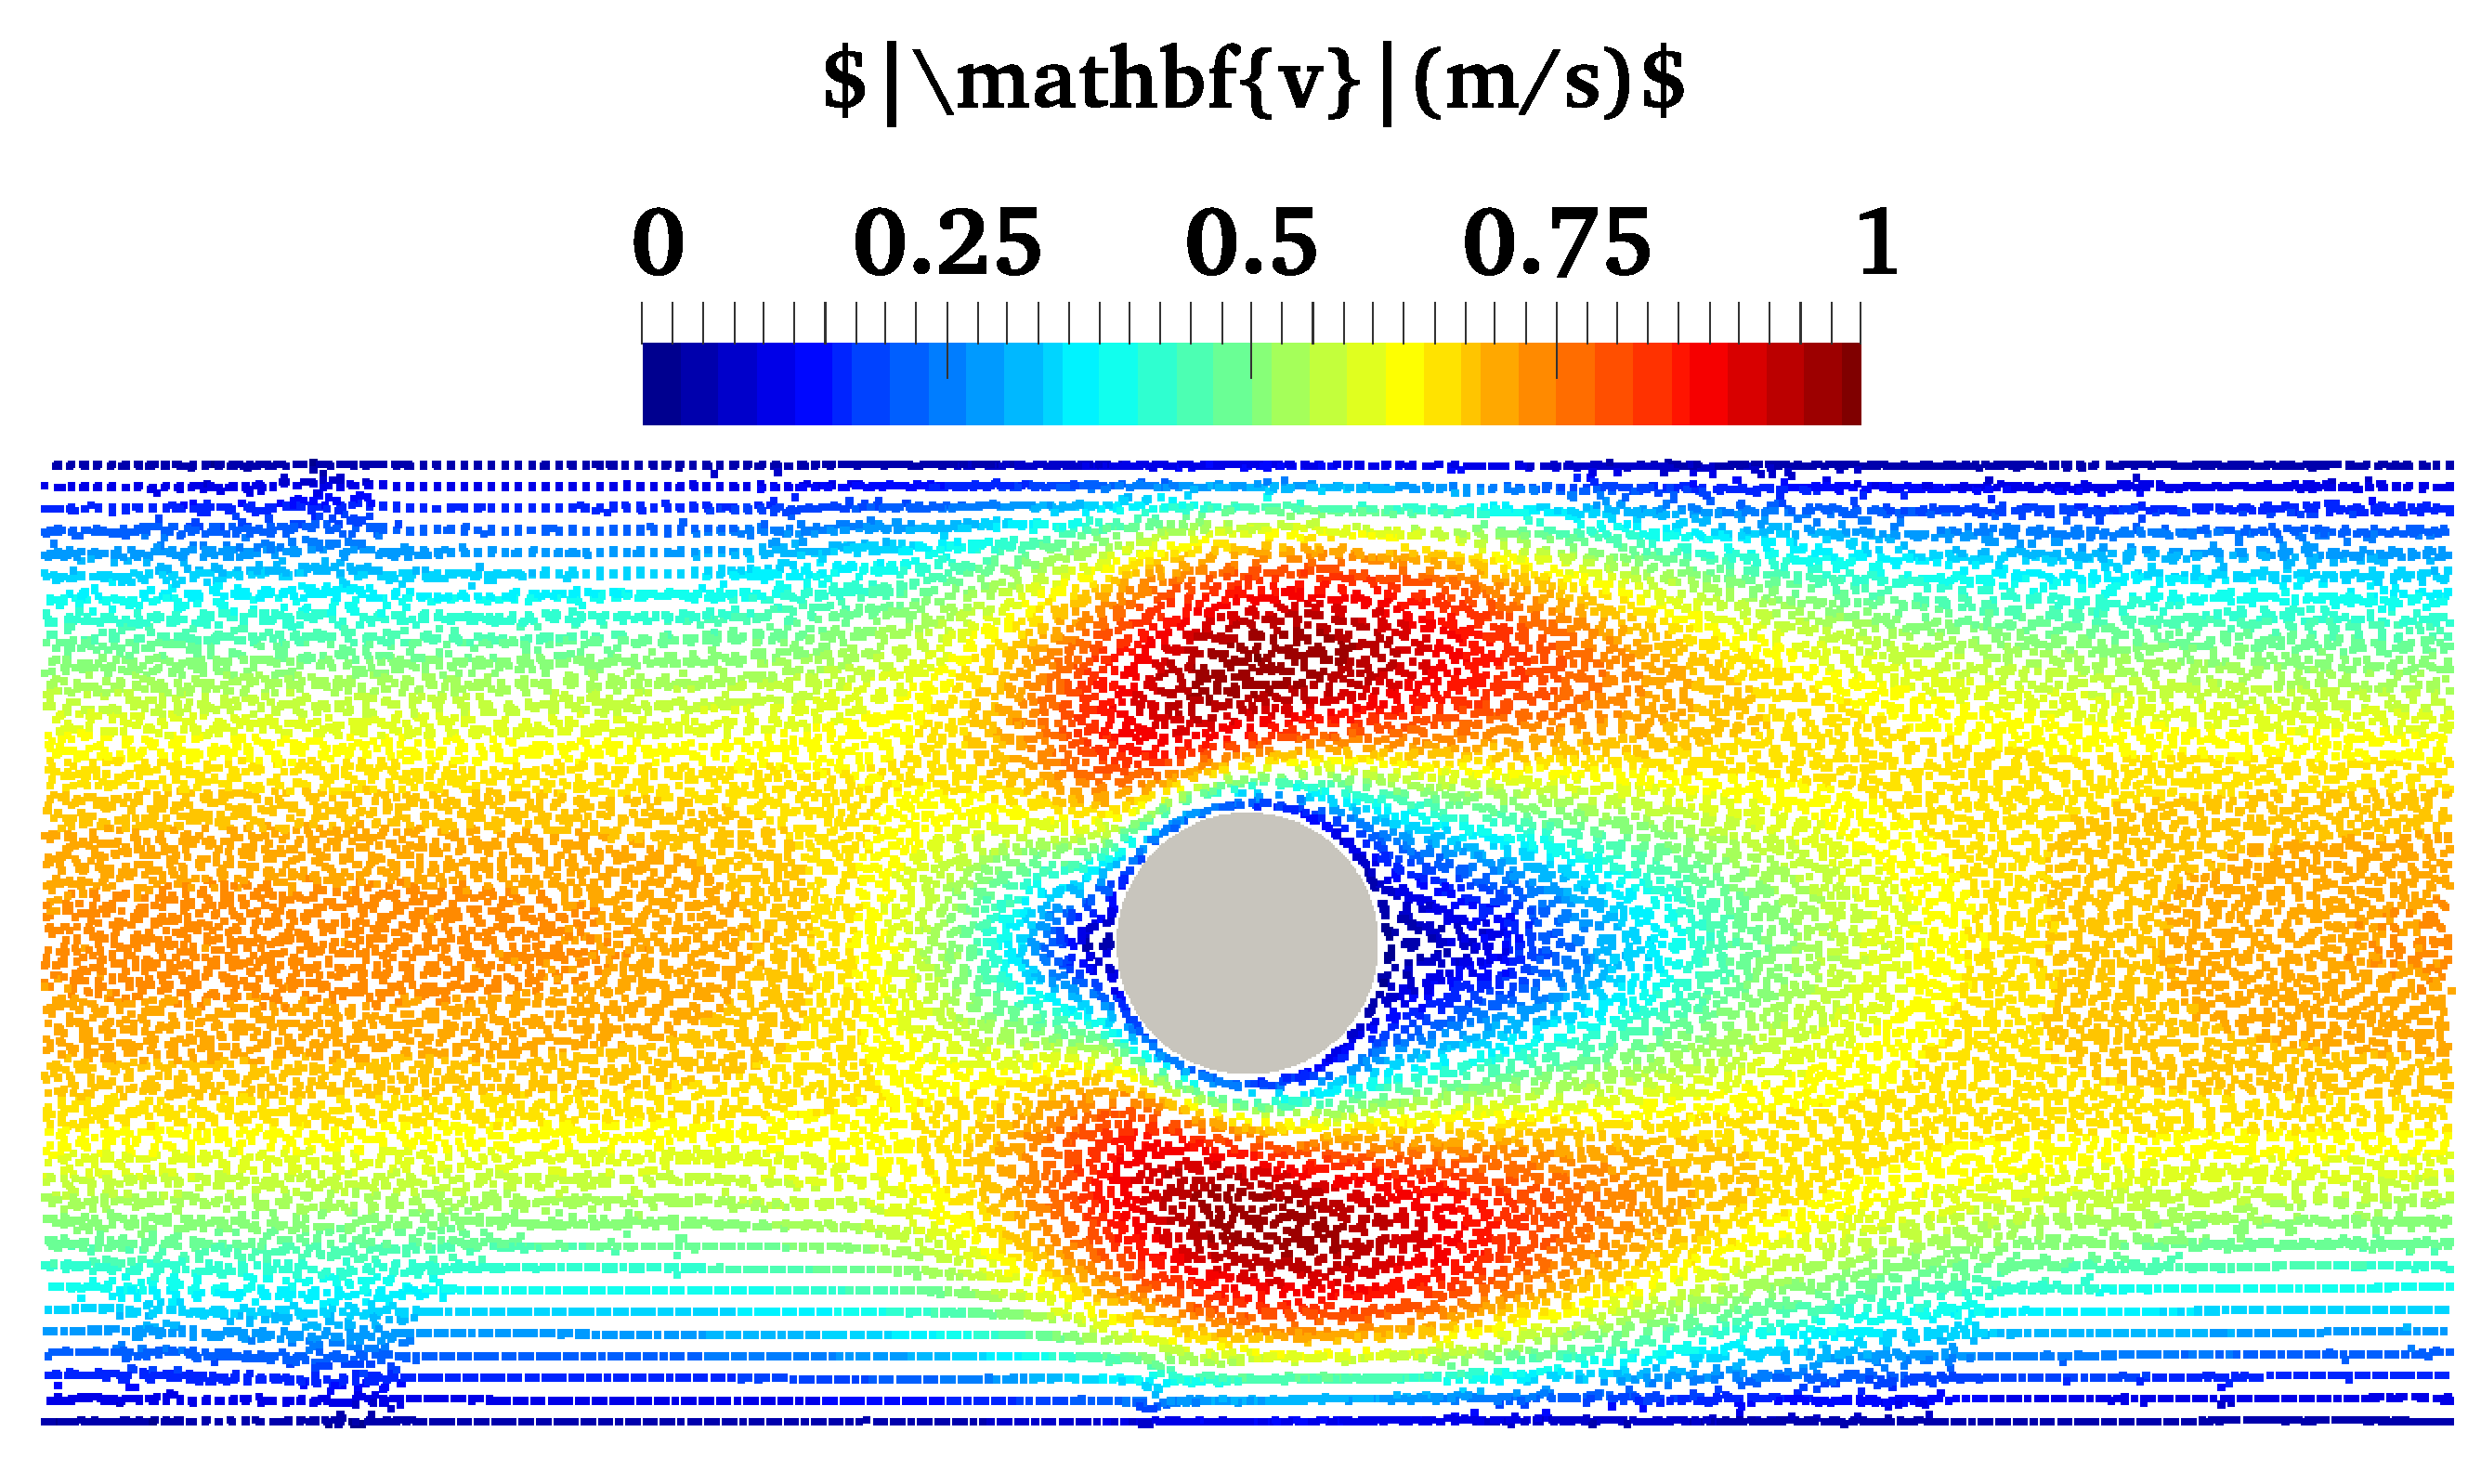
\includegraphics[width=1.0\textwidth]{images/SPH_Comparison/v_xsph.png}
	\end{subfigure}
	\begin{subfigure}{0.47\columnwidth}
		\centering
		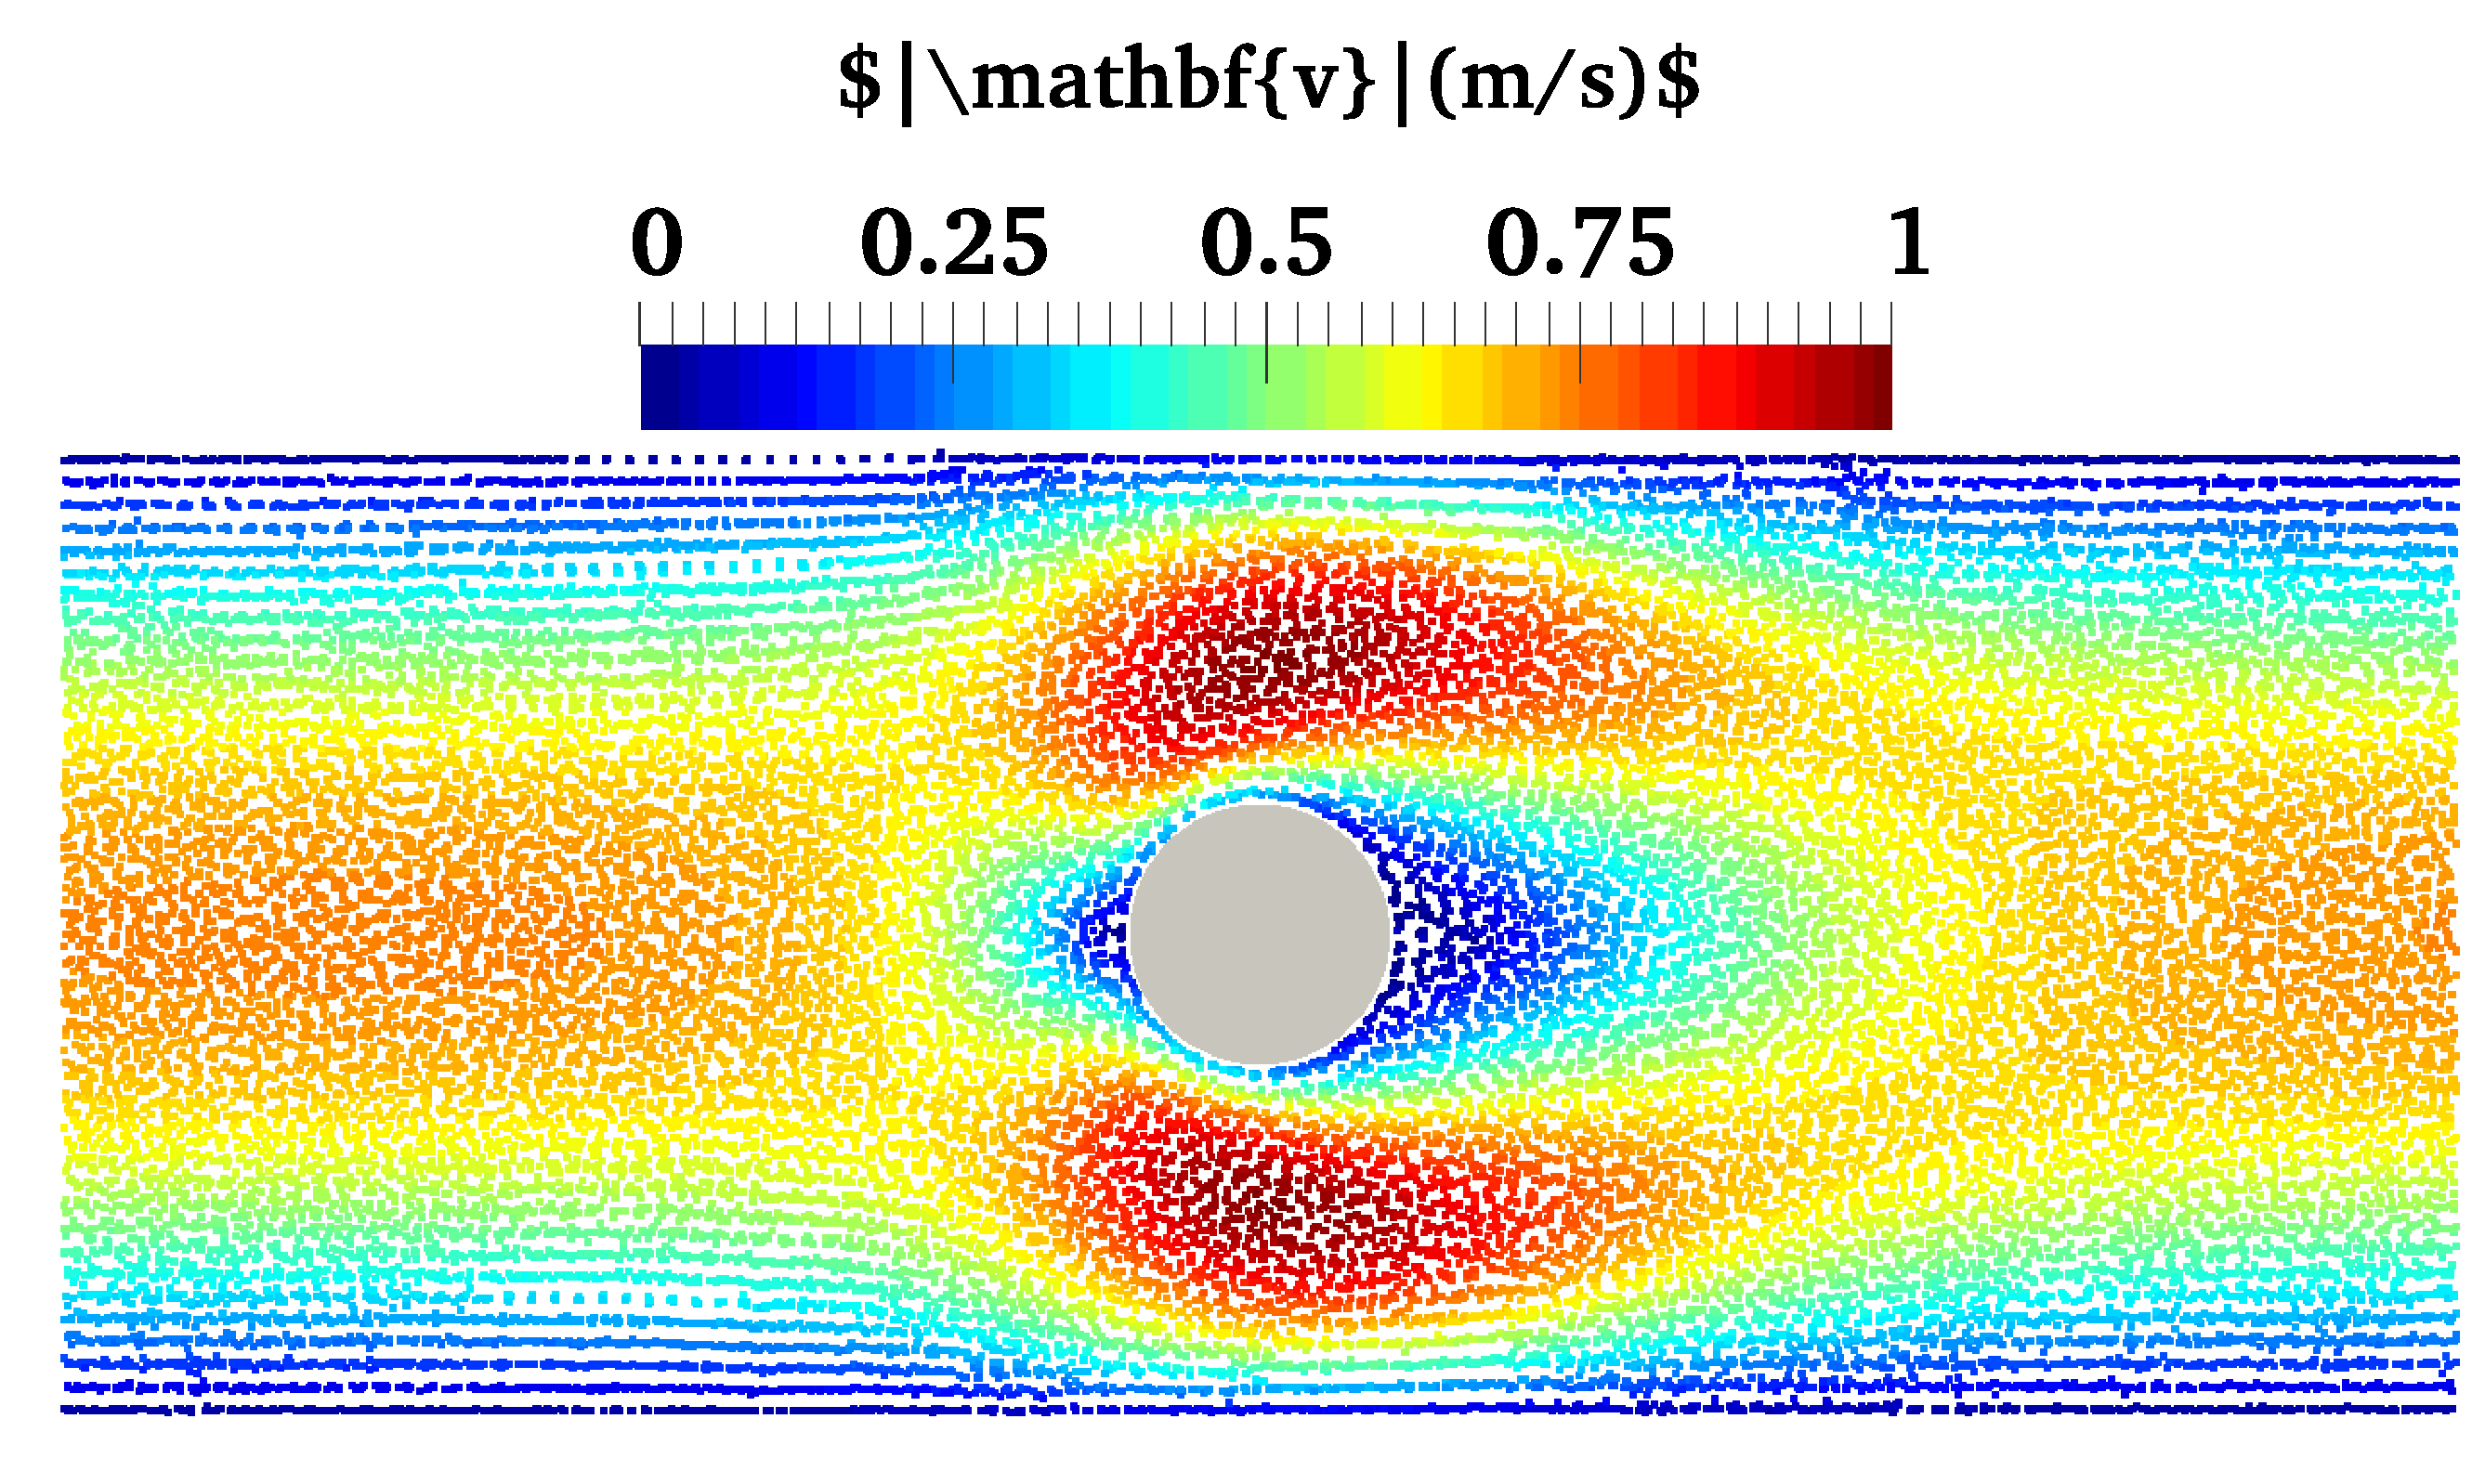
\includegraphics[width=1.0\textwidth]{images/SPH_Comparison/v_isph.png}
	\end{subfigure}
	\caption{Comparison of the steady-state velocity profiles predicted with WCSPH (left) and ISPH (right).}    \label{fig:FoCV}
\end{figure} 


We also note that there is no unique ISPH solution for pressure when solving the Poisson equation under pure Neumann boundary conditions -- in fact, the pressure solution is unique up to a constant. In other words, in the absence of Dirichlet boundary conditions, pressure is a relative quantity in the Navier-Stokes equations. Whereas the reference (\textit{minimum}) pressure for WCSPH is often set to zero, in ISPH, we choose the pressure solution with the \textit{average} value of zero.
Consequently, the difference between the legend of the plots in Fig.~\ref{fig:FoCP} has no real significance as long as the difference between the solutions is a constant offset that only indicates a reference pressure. Note that the choice of the reference pressure does not affect the gradient of the pressure, which is the quantity that comes into play in the Navier-Stokes equation.

\begin{figure}
	\centering    
	\begin{subfigure}{0.47\columnwidth}    
		\centering
		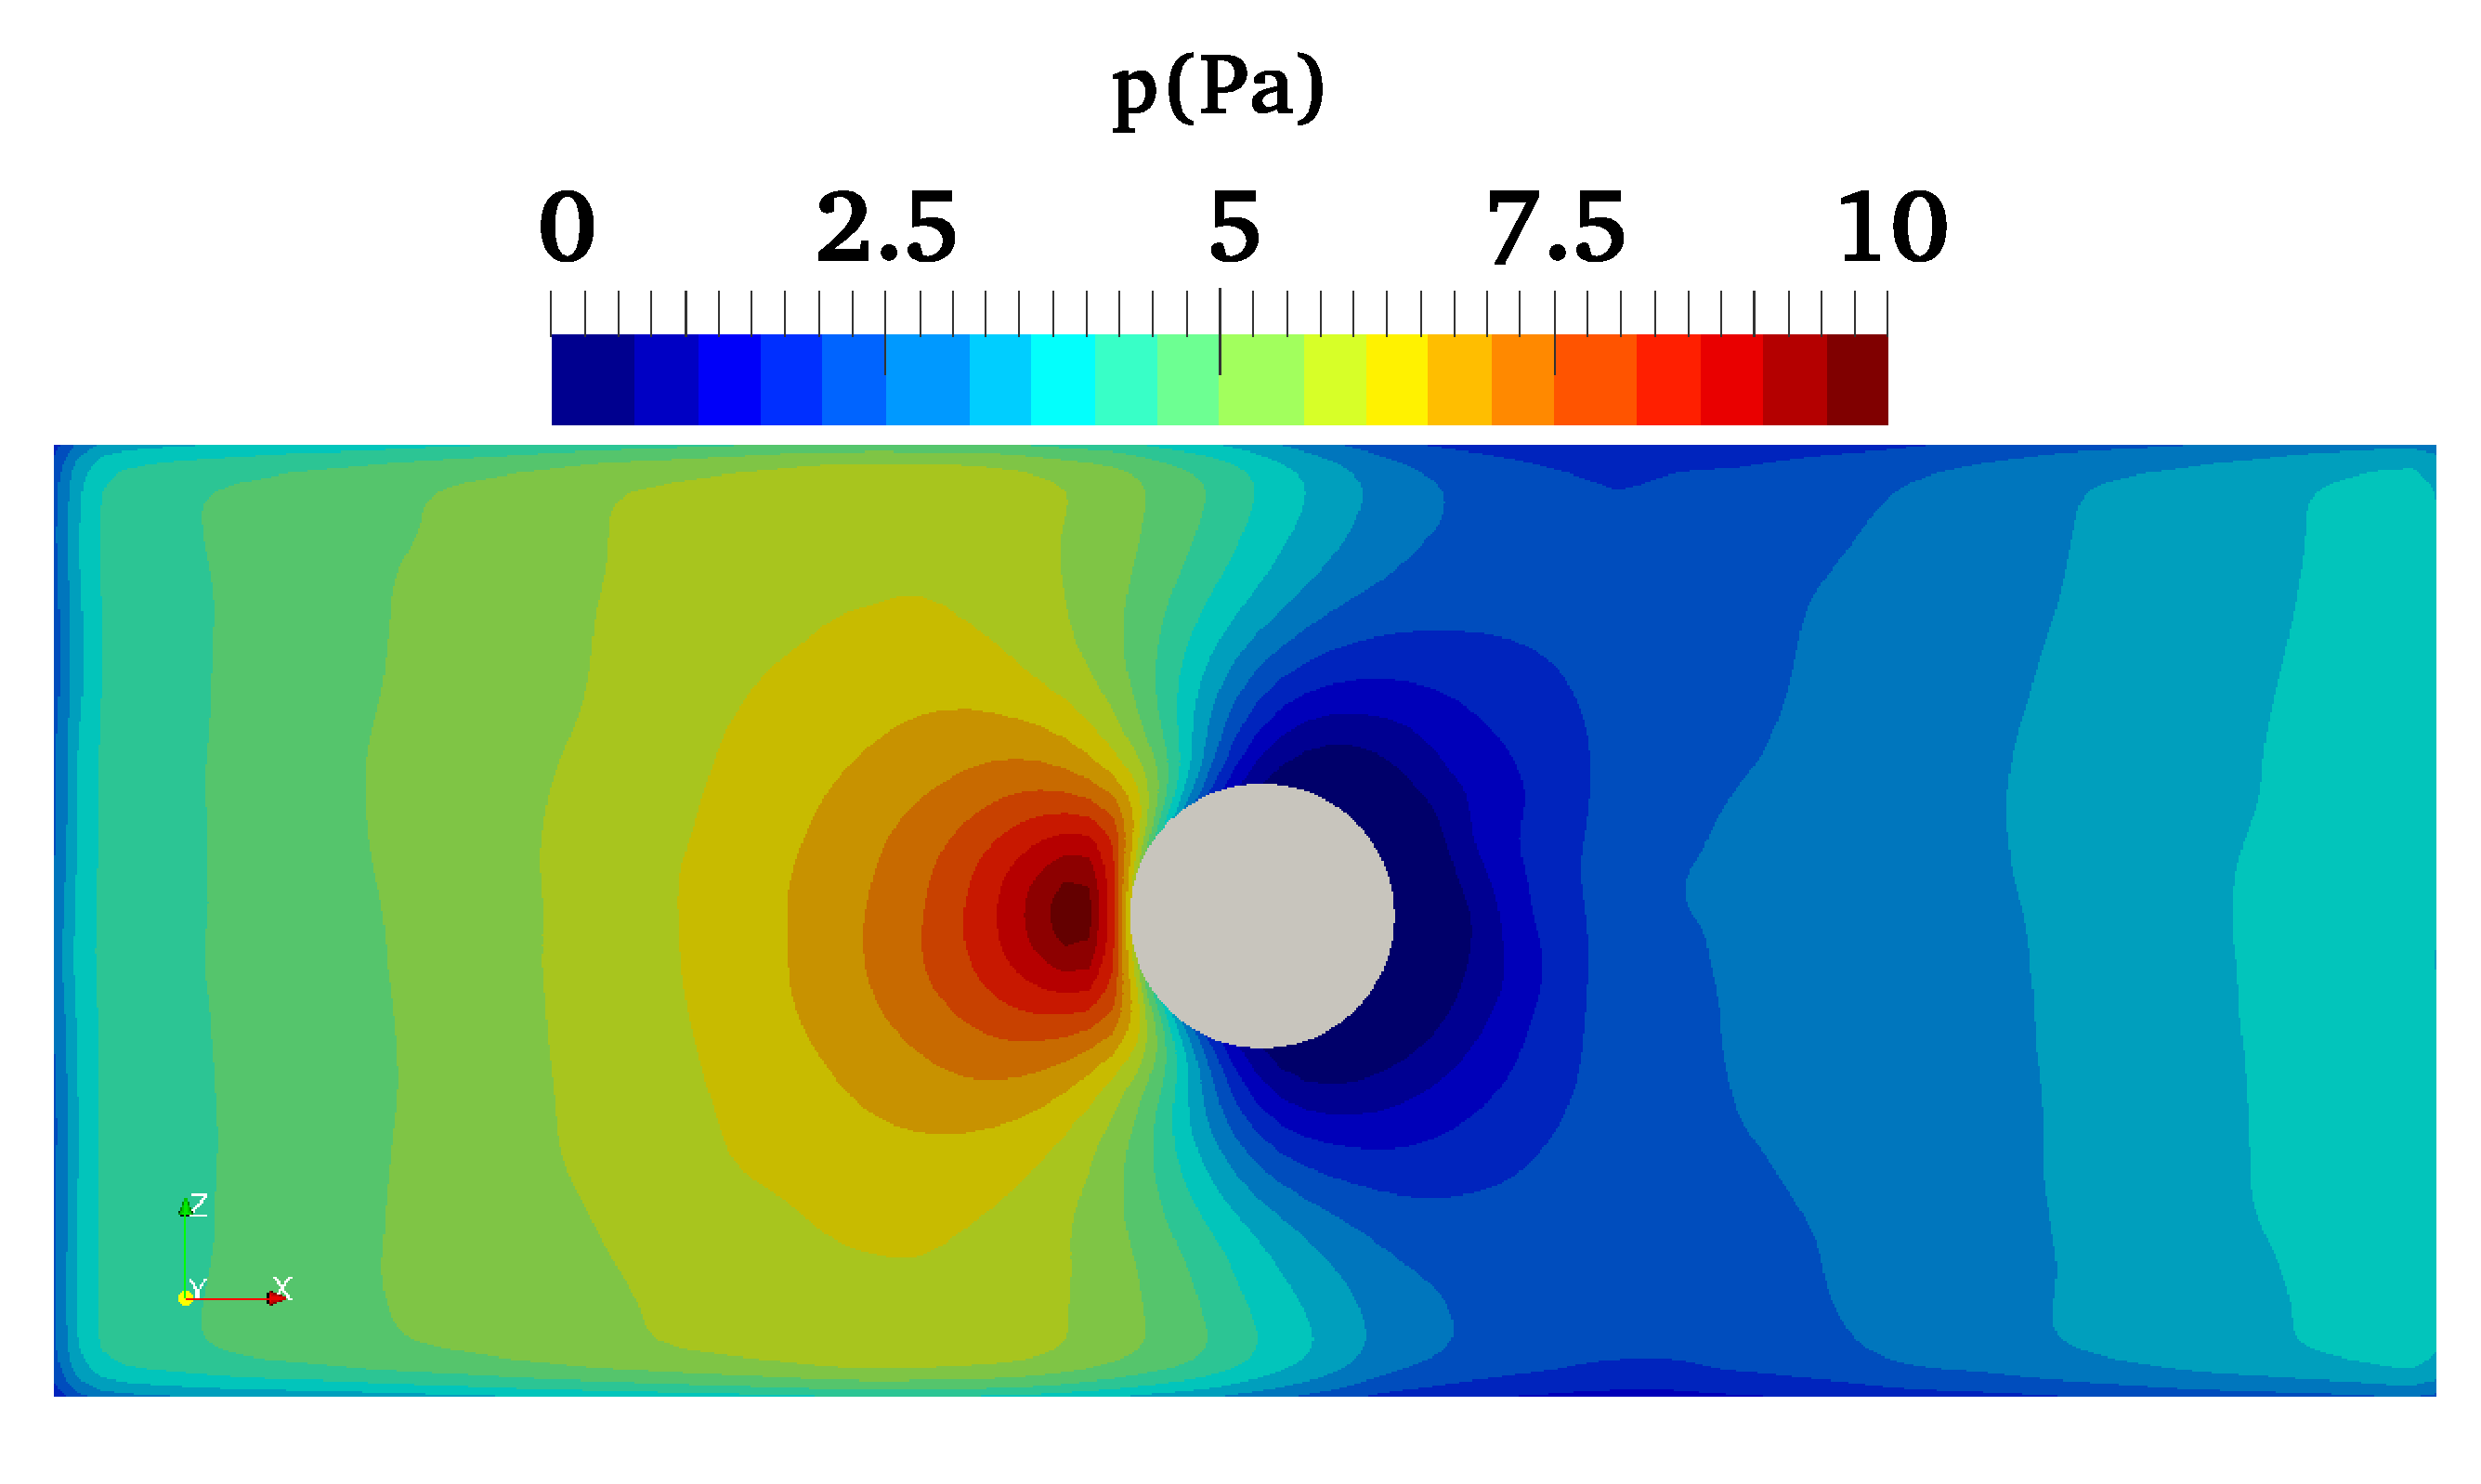
\includegraphics[width=1.0\textwidth]{images/SPH_Comparison/p_xsph.png}
	\end{subfigure}
	\begin{subfigure}{0.47\columnwidth}
		\centering
		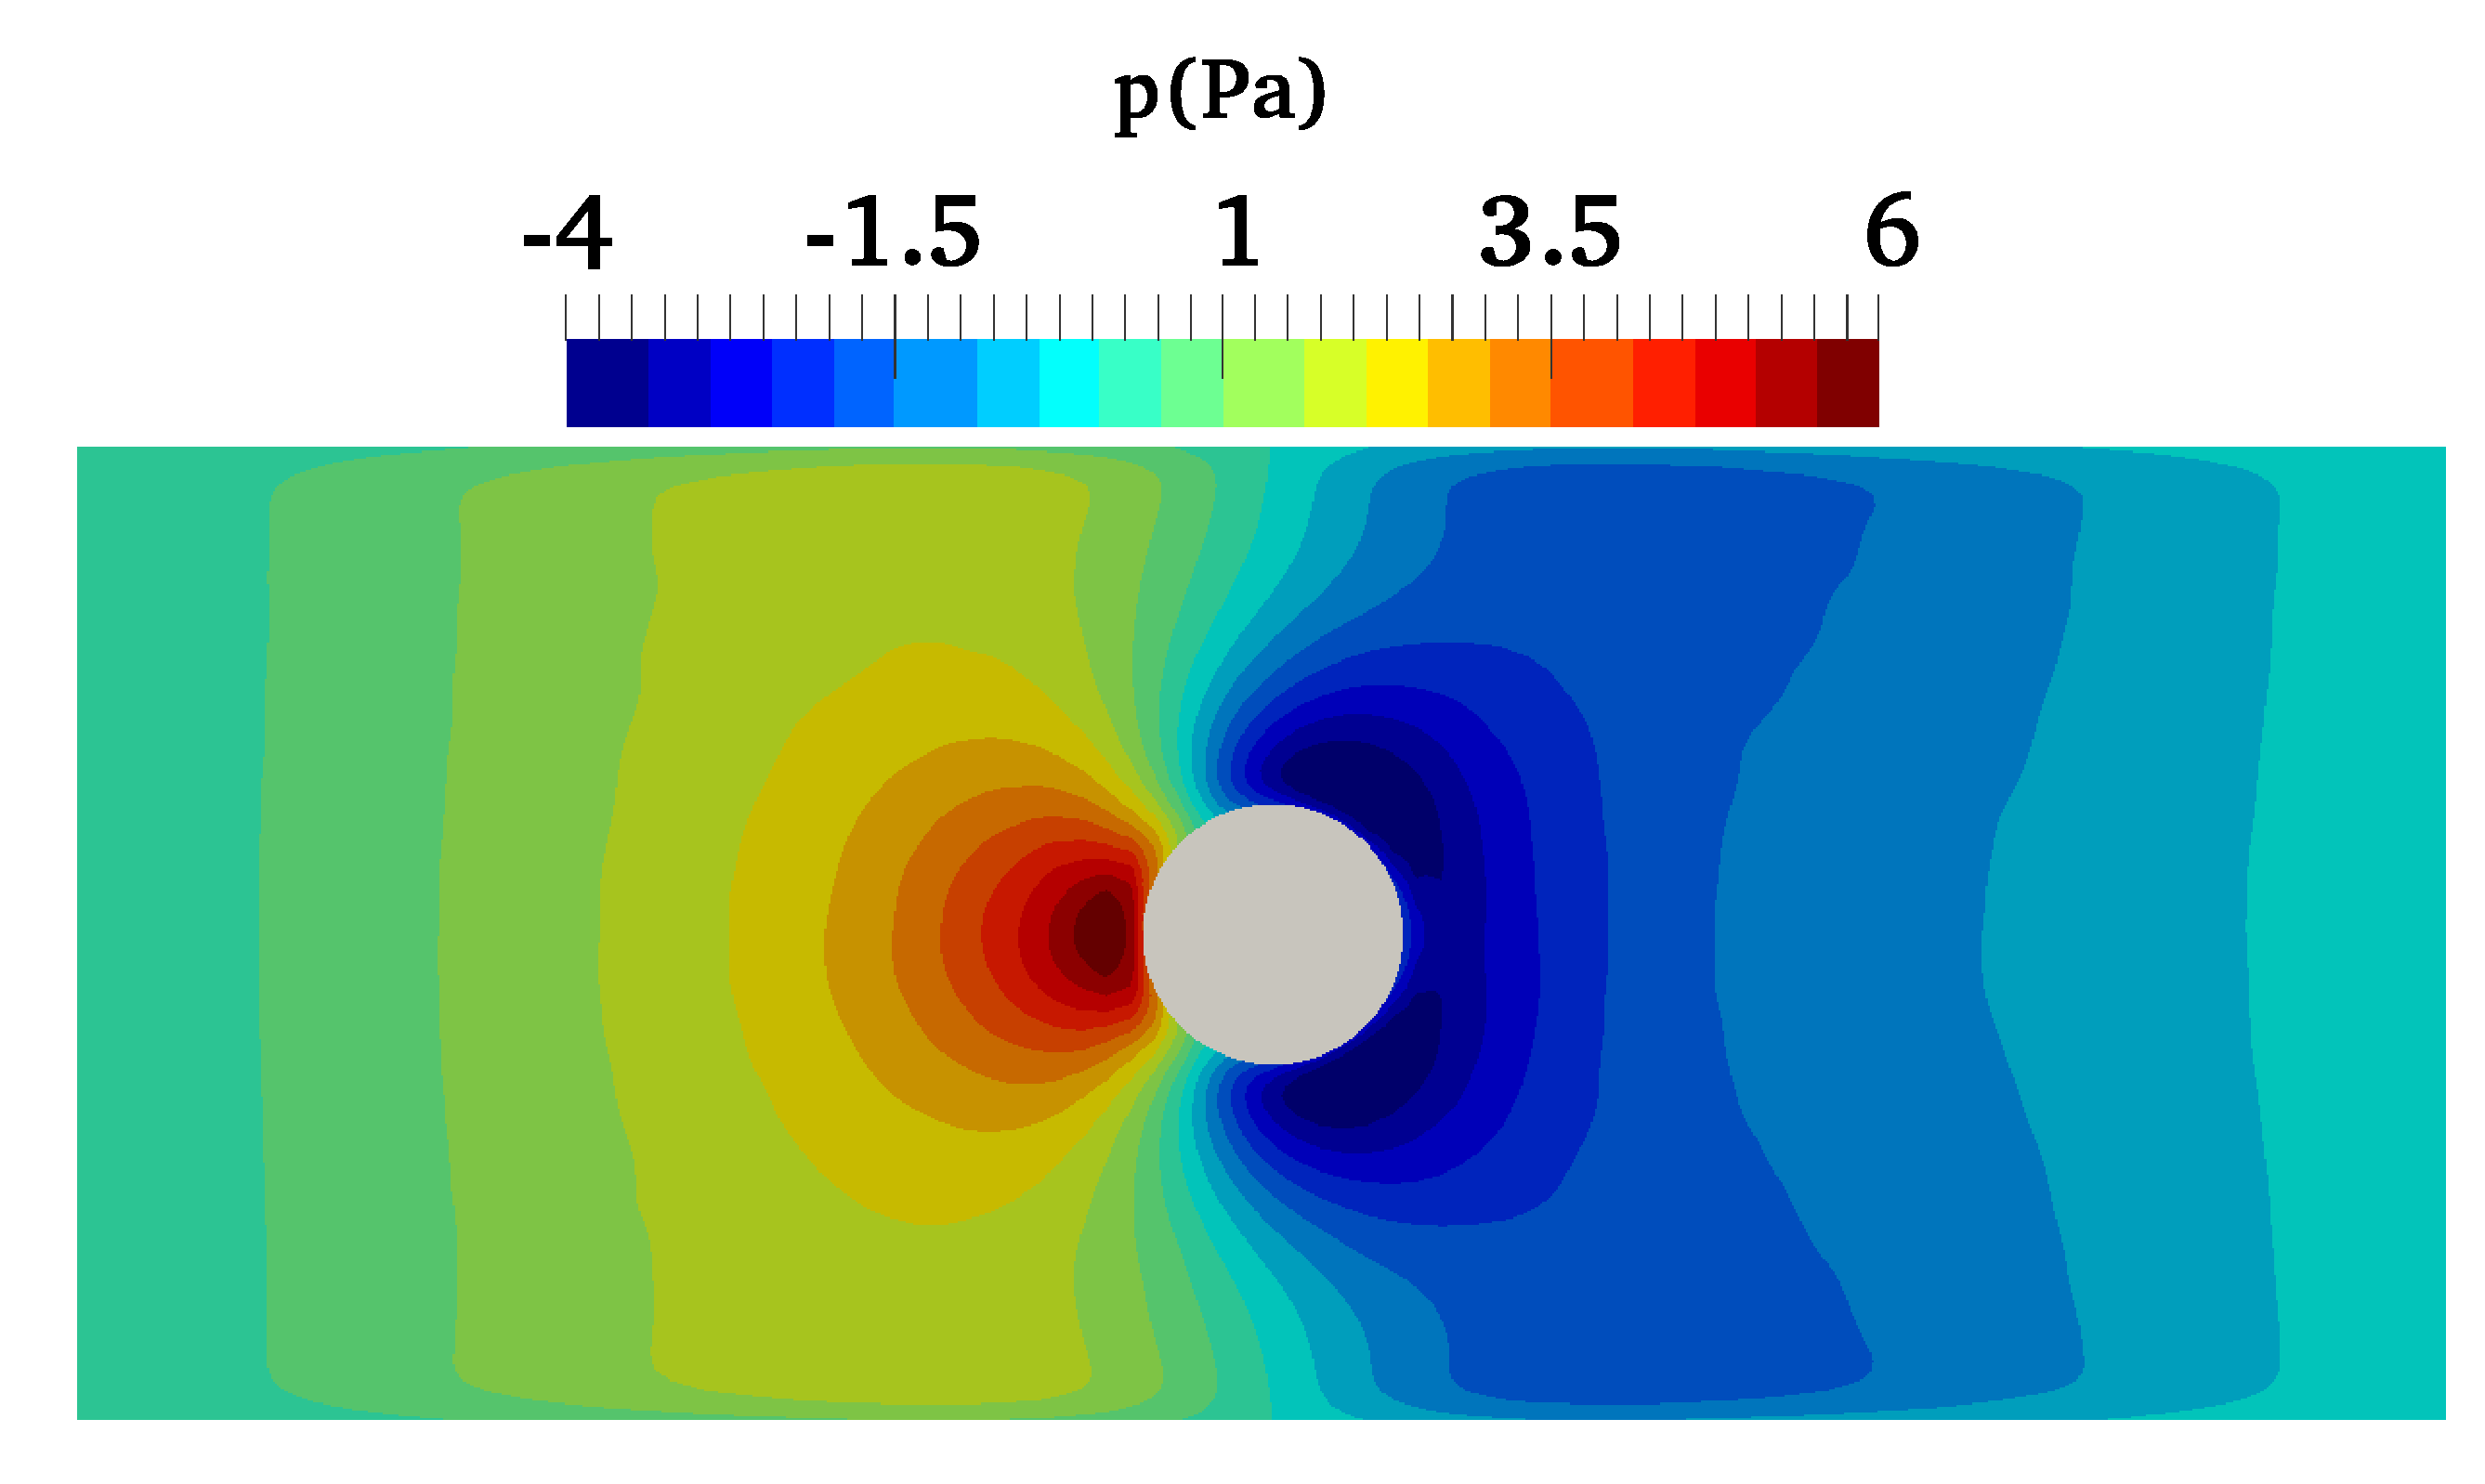
\includegraphics[width=1.0\textwidth]{images/SPH_Comparison/p_isph.png}
	\end{subfigure}
	\caption{Comparison of the steady-state pressure profiles predicted with  WCSPH (left) and ISPH (right).}    \label{fig:FoCP}
\end{figure} 
Herein, the expression used for the drag coefficient is $C_d=\frac{F_d}{0.5\rho\;A\; U^2}$, where $F_d$ is the drag force magnitude along the $x$ axis, $\rho=\rho_0$ and $U=1$\si{m/s} are the reference density and velocity, and $A$ is the frontal area of the cylinder. Comparing drag coefficient results is insightful since this exercise provides a macro-scale perspective that, while looking past micro-scale fluctuations, captures emergent behavior of practical relevance. As shown in Fig.~\ref{fig:FoC}, ISPH and WCSPH show different drag coefficients at the onset of the simulation yet the steady state solutions are in good agreement -- the relative error of the time-averaged drag coefficient over the last 2\si{s} of the simulations is $6.4$\%. We posit that two reasons contributing to these discrepancies are: ($i$) the different time-integration schemes used in the formulations (see Sections~\S\ref{sec:ISPH} and \S\ref{sec:WCSPH}), each with its own amount of numerical damping \cite{hairer2009odeBook}; and ($ii$) the vastly different treatment of the pressure by the two formulations.

\begin{figure}
	\vspace{-20pt}
	\begin{center}
		\includegraphics[width=0.5\textwidth]{images/SPH_Comparison/Figure_flow_around_cylinder.png}
	\end{center}
	\vspace{-10pt}
	\caption{Variation of the drag coefficient over time.}
	\label{fig:FoC}
\end{figure}


\subsection{Dam Break}
\label{subsec:damBreak}
Lagrangian methods such as SPH use the dam break benchmark test to assess the performance of fluid solvers in conjunction with a high transients, free-surface problem \cite{Martin1952,colagrossi2003numerical,hughes2010comparison,xu2016improved,miladHalfImplicit2018}. The fluid domain is a rectangular prism of size 2.0\si{m} $\times$ 0.5\si{m} $\times$ 1.0\si{m} consisting of \SI{64000} SPH particles that are placed on a regular lattice at $t=0$\si{s}. The reference density and viscosity are $\rho_0=1000$\si{kg/m^3} and $\mu=$\SI{0.001}{Pa.s}. The gravity $g=-9.8$\si{m/s^2} is applied in the  $z$ direction. The WCSPH, ISPH, and KCSPH results are compared from two perspectives: $(i)$ the fluid front position over time, and $(ii)$ the roll up and the second splash -- two characteristics highlighted in previous studies \cite{colagrossi2003numerical,Adami2012}. Figure~\ref{fig:db_front} shows the fluid front position as a function of time. While the KCSPH solution slightly over-estimate the front speed (no dissipation term is implemented in KCSPH), nearly identical front propagation is predicted by WCSPH and ISPH. 
\begin{figure}%[H]
	%    \vspace{-15pt}
	\begin{center}
		\includegraphics[width=0.5\textwidth]{images/SPH_Comparison/Figure_damBreak.png}
	\end{center}
	\vspace{-10pt}
	\caption{Comparison of water-front propagation between between KCSPH (top), WCSPH (middle), and ISPH (bottom).}
	\label{fig:db_front}
\end{figure}
With regard to the roll-up and second splash characteristics, all three methods predict well these two hallmark features of the dam break experiment, see Fig.~\ref{fig:db_charac}.
\begin{figure}[H]
	\centering    
	\begin{subfigure}{0.35\columnwidth}    
		\centering
		\includegraphics[width=1.0\textwidth]{images/SPH_Comparison/colorBar.png}
	\end{subfigure}
	
	\begin{subfigure}{0.4\columnwidth}    
		\centering
		\includegraphics[width=1.0\textwidth]{images/SPH_Comparison/cf_1.png}
	\end{subfigure}
	\begin{subfigure}{0.4\columnwidth}
		\centering
		\includegraphics[width=1.0\textwidth]{images/SPH_Comparison/cf_2.png}
	\end{subfigure}
	\begin{subfigure}{0.4\columnwidth}    
		\centering
		\includegraphics[width=1.0\textwidth]{images/SPH_Comparison/xsph_1.png}
	\end{subfigure}
	\begin{subfigure}{0.4\columnwidth}
		\centering
		\includegraphics[width=1.0\textwidth]{images/SPH_Comparison/xsph_2.png}
	\end{subfigure}
	\begin{subfigure}{0.4\columnwidth}    
		\centering
		\includegraphics[width=1.0\textwidth]{images/SPH_Comparison/isph_1.png}
	\end{subfigure}
	\begin{subfigure}{0.4\columnwidth}
		\centering
		\includegraphics[width=1.0\textwidth]{images/SPH_Comparison/isph_2.png}
	\end{subfigure}
	\caption{Comparison of the roll-up ($t=1.75$\si{s}, left) and the second splash ($t=2.05$\si{s}, right) characteristics between KCSPH (top), WCSPH (middle), and ISPH (bottom).}    
	\label{fig:db_charac}
\end{figure}

\subsection{Sloshing}
Sloshing probes the ability of a CFD solver to handle a free-surface problem that experiences lower frequency transients (when compared to the dam break). In this experiment a fluid container undergoes a forced vibration motion according to $X_0 = sin(2\pi f t)$, where $t$ is time, and $f$ and $X_0$ are the frequency and the amplitude of the vibration, respectively. The analytical solution of this problem under the inviscid flow assumption was discussed in \cite{Dodge2000} and involves a set of natural frequencies $\omega_n$ defined as
\[
\omega_n^2 =\left(2n-1\right) \pi \left(\frac{g}{w}\right) \text{tanh} \left[\left(2n-1\right) \pi \left(\frac{h}{w}\right)\right],
\]
where $n$ is the mode number, $g$ is the value of the gravitational acceleration, $w$ is the tank width; i.e., the tank dimension in the direction of oscillation, and $h$ is the height of the fluid at rest. The analytical amplitude $F_{x_0}$ of the net force exerted by the fluid on a sloshing tank in a forced vibration can then be expressed as 
\begin{equation*} 
\frac{F_{x_0}}{\Omega^2 X_0 m_l} = 1 + 8\frac{w}{h} \sum_{n=1}^{N} \frac{\text{tanh}\left[\left(2n-1\right) \pi h / w\right]}{\left(2n-1\right)^3 \pi ^3} \frac{\Omega ^2}{\omega_n^2 - \Omega^2} \;.
\end{equation*}
Above, $\Omega=2\pi f$ is the frequency of the oscillation and $m_l$ is the mass of the liquid. The exerted force on the container in the horizontal direction is expressed as  $F_x=F_{x_0} sin(2\pi f t)$.

We compare the ISPH, WCSPH, and KCSPH approximations with the analytical solution for the following problem: the dimension of the domain ($w \times b \times h$) is  1.2\si{m} $\times$ 0.4\si{m} $\times$ 1.7\si{m} and the  fluid density is $\rho_0=1000$\si{kg/m^3}. The gravity $g=-9.8$\si{m/s^2} is applied in the  $z$ direction. The numerical model is comprised of 98k SPH markers, which are placed on a uniform Cartesian lattice at $t=0$\si{s}. The frequency and amplitude of the vibration are set to be $f=0.75$\si{s^{-1}} and $X_0=0.1$\si{m}.  Figure~\ref{fig:Sloshing} reports the sloshing force exerted on the container over time. 
\begin{figure}[H]
	\begin{center}
		\includegraphics[width=0.7\textwidth]{images/SPH_Comparison/Figure_Sloshing.png}
	\end{center}
	\caption{Sloshing experiment: Comparison of fluid-structure interaction force along the axis of periodic motion.}
	\label{fig:Sloshing}
\end{figure}

Ignoring the initial transient period, all methods predict the dynamic interaction forces with reasonable accuracy. We attribute the initial discrepancy between the numerical and the analytical solutions to the fact that the simulation tank starts its motion from rest; hence the initial condition of the simulation is different from the analytical solution, the latter only reported in the steady-state regime. However, the initial transient motion is damped in approximately 1 \si{s}. As shown in Fig.~\ref{fig:Sloshing}, the steady-state solution of ISPH closely matches the analytical solution; the steady-state solution of the WCSPH slightly over-predicts, whereas the KCSPH solution under-predicts the analytical result.

\subsection{Discussion}\label{sec:discussion_SPHs}
This effort set out to gauge the agency of the SPH methodology, employed here in conjunction with three approaches to time stepping and incompressibility enforcement. WCSPH uses an equation of state for pressure along with explicit time stepping. ISPH falls back on a Poisson problem to enforce incompressibility Chorin-style time stepping. KCSPH enforces incompressibility via a kinematic constraint that asserts the constant value of the density while a half-implicit symplectic Euler integrator is used for time stepping. 

\vspace{3pt}

\noindent \textit{WCSPH, ISPH, KCSPH: Ease of implementation comments.} WCSPH and ISPH leveraged GPU computing through CUDA; KCSPH used multi-core parallel computing via OpenMP \cite{openMP}. The amount of effort required to implement these solvers in software was quite different. Implementing the WCSPH solver was easier than ISPH, which was easier than KCSPH. ISPH requires the solution of a sparse linear system on the GPU; such a solver is not readily available and herein, the implementation resorted to Krylov subspace iterative methods such as BICGSTAB and GMRES \cite{saad1989overview}. A memory-efficient solver requires sparse storage of the underlying systems (see Eqs.~\ref{eq:U_BC} and \ref{eq:p_BC}). Assembling and solving these sparse linear systems made the ISPH implementation nontrivial. KCSPH was more challenging to implement since it required at each integration step the solution of a constrained quadratic optimization problem, see \cite{hammadConstrFluid2018}. This optimization problem was posed in hundreds of thousands of variables -- as many as SPH particles used in the formulation and its solution was found using a Nesterov-type method \cite{hammadTOG2015}. 

\vspace{3pt}

\noindent \textit{WCSPH, ISPH, KCSPH: Solution robustness comments.}
KCSPH and ISPH  provide more robust (as in less finicky) solutions due to the coupling they establish between the field variables. Owing to the integration scheme used in ISPH, the velocity and pressure/density are coupled more tightly than in WCSPH, where pressure depends only on the density. Similarly in KCSPH, the pressures, which are a proxy of the Lagrange multipliers for the density kinematic constraints, are coupled with the velocity in a fully implicit sense. 

\vspace{3pt}

\noindent \textit{WCSPH, ISPH, KCSPH: Solution quality comments.} A simple answer to the question ``which method provides better quality results?'' is difficult to provide as multiple factors come into play in determining the quality of the solution, e.g., the particle resolution, the consistency vs. conservancy dichotomy, the decision to use or not particle shifting, the size of the time step, the nature of the problem solved, etc. This question is brought more into focus by stating that the interest is in obtaining results that are insightful without taxing tinkering with parameters, settings, etc. In general, ISPH turned out to be easier to set up and get good results with. It is robust (non-finicky) and for a given simulation time budget, it provides better quality results. One stumbling block is that ISPH requires a sparse linear solver. WCSPH, particularly for the non-consistent version, usually yields more noisy results -- this also came through in the flow-around-the-cylinder test. KCSPH shows potential, but it needs further investigation to improve the handling of viscosity and reduce execution speed as it requires the solution of a constrained convex optimization problem.

\vspace{3pt}

\noindent \textit{WCSPH, ISPH, KCSPH: Time to solution comments.}
While an efficiency comparison of WCSPH, ISPH, and KCSPH falls outside the scope of this contribution owing to the sheer scope of such an undertaking, we considered insightful to provide timing results to understand, insofar as order of magnitude is concerned, how long an SPH simulation would take. The problem considered was the dam break simulation of \S\ref{subsec:damBreak}. There was no attempt to optimize the WCSPH, ISPH, and KCSPH implementations, which were made in Chrono. Therein, WCSPH and ISPH rely on GPU computing; KCSPH draws on OpenMP. %We find this {\textit{qualitative}} information useful to understand, as order of magnitude, simulation times associated with this benchmark SPH problem. 
Table~\ref{tab:speed} shows {\textit{qualitative}} information regarding the first second of simulation of the dam break problem. All 3D solvers used \SI{215000} SPH markers. WCSPH takes smaller step sizes due to the explicit time stepping. However, its effort per time step is both step-size independent and cheaper than for ISPH or KCSPH. For the latter two, given the iterative nature of the solution process, higher computational costs are incurred for larger step sizes. Note that even for the same integration time step, the amount of time required to converge at different points in the ISPH/KCSPH simulation might be different owing to the difference in the number of iterations that the underlying linear system/optimization solvers require to converge. 
\begin{table}\centering
	\begin{tabular}{cccc}
		\toprule
		
		method & $\Delta t$(\si{s}) &  simulation time (\si{s}) & average time per step (\si{s})\\
		\midrule
		
		WCSPH & $10^{-4}$ & 1646 & 0.17 \\
		WCSPH & $2.5\times 10^{-4}$ & 682 & 0.17 \\
		ISPH & $10^{-3}$ & 1692 & 1.69 \\
		ISPH & $5\times 10^{-3}$ & 369 & 1.84 \\
		
		KCSPH & $10^{-3}$ & 1523 & 1.52 \\
		KCSPH & $5\times 10^{-3}$ & 531 & 2.65 \\
		\bottomrule
	\end{tabular}
	\caption{Dam break, qualitative information: solver execution times for the first second of the simulation.}
\end{table}\label{tab:speed}

\vspace{3pt}

\noindent \textit{WCSPH, ISPH, KCSPH: Use case recommendations.}
WCSPH is the method of choice for many single-phase and free-surface CFD problems such as the dam break and Poiseuille flow. ISPH was found to be a better choice when more complex physics, e.g., vortex shedding, boundary layer separation, etc., are present. This is the case for problems like flow around cylinder and the flow over backward facing step at higher Reynolds numbers ($Re\approx 10^2$--$10^3$). ISPH is also the solver of choice for FSI problems with relatively simple boundary geometries. KCSPH leverages multi-body dynamics approaches, which opens the door to monolithic frameworks for more involved FSI problems, e.g., fording scenarios with complex vehicle models (wheeled, tracked) \cite{hammadConstrFluid2018}. Indeed, imposing ISPH or WCSPH boundary conditions on a complex mesh, e.g., a vehicle, requires a uniformly generated point cloud, whereas KCSPH does not have this restriction and is more flexible in terms of boundary condition enforcement. 

%\vspace{3pt}
%
%\noindent \textit{WCSPH, ISPH, KCSPH: Connections to other physics.} The inspiration for the KCSPH method used in this study is a granular dynamics solution approach. Indeed, WCSPH has a granular dynamics twin in the discrete element method (DEM) \cite{cundall79}. However, there is a second class of granular dynamics methods that belongs to the family of ``contact dynamics'' or differential variational inequality approaches, in which the non-penetration condition is enforced by kinematic constraints, see, for instance \cite{negrutSerbanTasoraJCND2017}. The ``contact dynamics'' twin in fluid dynamics would be one that explicitly states that $\rho(t) = \rho_0$; i.e., KCSPH. Continuing this granular dynamics--fluid dynamics parallel, the analog of the contact force in granular dynamics is the pressure in fluid dynamics; likewise, the friction force at the contact between two grains is the twin of the shear force in fluid dynamics. Another salient point in this analogy is that the pressure in ISPH is the analog of the Lagrange multiplier that enforces the $\rho(t) = \rho_0$ in KCSPH, made clear in this contribution by casting the SPH spatial discretization in a matrix-vector form. This is unsurprising given that in an incompressible, Newtonian fluid model the pressure is devoid of a thermodynamic trait and instead becomes a mechanical attribute of the flow. For Newtonian fluids though, the analogy ends here -- while for a Newtonian fluid the shear force only depends on velocity, in granular dynamics the friction force is tied to the contact (normal) force through a yield condition that caps the former at a value equal to the normal force scaled by $\mu$, the friction coefficient: $f_f \leq \mu f_n$.





\section{IISPH Method}\label{sec:IISPH_Val}
\subsection{Incompressibility Test}
\label{subsec:incompressibilityTest}
In this test we monitor the value of the density over time for a fluid stored in a container. A rectangular container with dimensions \SI{1.1}{m} (L) $\times$ \SI{1.1}{m} (W) $\times$ \SI{1.2}{m} (H) is initialized with fluid particles. The particles are free to move inside the container under the influence of viscous and gravitational forces. We seek to understand how successful the IISPH solution implemented is in enforcing the incompressibility condition. The reference WCSPH solution is provided by the open-source software DualSPHysics  \cite{crespo2015dualsphysics}. In DualSPHysics, the maximum CFL value was set to \num{0.1}, i.e. $C_{max}=0.1$, and the speed of sound $c_s$ was varied to obtain different levels of compressibility. Other settings were carried over from the dam break tutorial provided with DualSphysics \cite{crespo2015dualsphysics}. Both solvers used approximately \num{56000} SPH particles to include a \num{32}$\times$\num{32}$\times$\num{35} distribution of particles plus additional BCE particles. 

Figure~\ref{fig:Compressibility_Comparison} confirms that increasing $c_s$ in WCSPH leads to smaller density errors. However, the larger $c_s$, the stiffer the numerical problem, which translates into smaller integration step size. Thus, at one end of the spectrum, WCSPH uses small yet computationally inexpensive time steps. At the other end of the spectrum, IISPH allows for large albeit more computationally costly time steps. Against this backdrop, Fig.~\ref{fig:Compressibility_Comparison} answers the following question: what value of $c_s$ and $\Delta t_{WCSPH}$ should be used for DualSPHysics so that the quality of the solutions produced by IISPH and WCSPH are comparable? As shown in Fig.~\ref{fig:Compressibility_Comparison}, an approximately $100$-fold larger time step can be adopted by the IISPH method for the same level of compression. The vertical axis in the figure shows the relative error at every time step, which is defined, for the time step $(l)$ as
\[
\% \mbox{ error}^{(l)}  \equiv (\frac{1}{\rho_0 \nFluid } \sum_{i=1}^{\nFluid} \rho_i^{(l)} -1) \times 100 \; ,
\]
\noindent where $N_F$ is the number of SPH particles; in Fig.~\ref{fig:Compressibility_Comparison}, ``tol'' stands for the tolerance used in the linear solver. Recall though that the larger IISPH step size comes at the cost of solving a linear system of equations at each time step.
%\input{images/Compressibility.tex}
\begin{figure}[H]
	\begin{center}
		\includegraphics[width=0.9\textwidth]{images/IISPH/tikz/Compressibility.png}
	\end{center}
	\caption{IISPH vs. WCSPH (DualSPHysics \cite{crespo2015dualsphysics}) comparison based on the relative drift in the incompressibility.}
	\label{fig:Compressibility_Comparison}
\end{figure}

%\subsection{Dam Break}
%The dam break is often used to assess the performance of fluid solvers for free-surface simulation \cite{Adami2012,Martin1952,colagrossi2003numerical,hughes2010comparison}. The fluid behind the dam fits in a cube of $1$ \si{m} (height), $1$ \si{m} (width) and $0.5$ \si{m} (depth). The reference density is $\rho=1$ \si{kg/m^3}. At  $t=0$ \si{s}, the SPH particles are placed on a uniform Cartesian lattice. The gravity $g=1$ \si{m/s^2} is applied in the negative $y$. The approximate Reynolds number is $Re \approx 400$ \cite{Adami2012}. Upon conducting a particle resolution study with SPH characteristic lengths of $0.05$, $0.025$, $0.0125$ \si{m}, which resulted in \num{61000}, \num{245000}, and \num{1070000} SPH particles respectively, we observed the results are practically size-independent beyond the intermediate resolution. Good agreement between numerical results and experimental data \cite{Martin1952} is observed for $t<2$, see Fig.~\ref{fig:waterFront}. The simulation results slightly over-predict the experimental data after $t=2$, which is a trend reported in previous studies \cite{Adami2012,asai2012stabilized}. This discrepancy has been attributed to uncertainties resulting from several factors including lack of surface-tension model and the numerical viscosity formulation \cite{Adami2012}.
%\tikzsetnextfilename{waterFront}
\tikzset{external/export next=false}
\begin{figure}[H]
	\centering
	\begin{tikzpicture}
		\begin{axis}[
			width=0.6\columnwidth,
			%height=0.6\textwidth,
			xlabel = $t(gH)^{-1/2}$,
			ylabel = $x_{front}/H$,
			xmin=0, xmax=3.2,
			ymin=0, ymax=6,
			xtick={0,0.5,...,3},
			ytick={0,1,...,6},
			minor y tick num={1},
			minor x tick num={1},
			y tick label style={
				/pgf/number format/fixed,
				/pgf/number format/fixed zerofill,
				/pgf/number format/precision=1},
			axis x line=middle,
			axis y line=middle,			
			grid=both,
			grid style={dotted},
			%legend cell align = left,
			x tick label style={/pgf/number format/fixed},
			%no marks,
			]
			\addplot[black,very thick,,only marks, mark=o]
			table[
			x index={0},
			y index={1}, 
			]{images/Figs/Front_Pos_damBreak.txt};
			
			\addplot[black,very thick]
			table[
			x expr=\thisrowno{0},
			y expr=\thisrowno{1}+2.75, %This is the offset of the corner of the dam
			]{images/Analysis_DamBreak.txt};
			\legend{\small Martin and Moyce \cite{Martin1952},  \small Present Study}
			
			
\texttt{}%			\addplot[black,very thick,dashed,domain=0:4, samples=20]
%			{1.8*(x-0.45)};
%			\legend{\small Martin and Moyce \cite{Martin1952},  \small Present Study}
%					
		\end{axis}
	\end{tikzpicture}
%	\caption{Lift coefficient}
		\caption{Comparison of water-front propagation between IISPH  and experimental results of Martin and Moyce \cite{Martin1952,Shao2003}.}
			\label{fig:waterFront}
\end{figure}
%%\begin{figure}[H]
%%	\begin{center}
%%		\includegraphics[width=0.65\textwidth]{tikz/DamBreak.pdf}
%%	\end{center}
%%		\caption{Comparison of water-front propagation between IISPH  and experimental results of Martin and Moyce \cite{Martin1952,Shao2003}.}
%%\label{fig:waterFront}
%%\end{figure}
%
%Next, we compare our results with the classical dam break simulation discussed in \cite{colagrossi2003numerical}. To this end, the fluid height was $1$ \si{m}, width was $2$ \si{m}, and the size of the domain in which the fluid moved was $5.36$ \si{m}. The highlights of the dam break benchmark; i.e.,  the roll-up and the second splash \cite{colagrossi2003numerical,Adami2012}, can be captured by the current formulation as shown in Fig. \ref{fig:dambreak}. The simulation ran for 12 \si{s} and showed no instability issues. An animation of this simulation is available at \cite{sbelWebsiteAnimations} as movie \#139.
%
%\begin{figure}[t]
%	\vspace{-40pt}
%	\centering
%	\begin{subfigure}{0.3\columnwidth}	
%		\centering
%		\includegraphics[width=1.0\textwidth]{images/IISPH/Color_Dambreak.png}
%	\end{subfigure}
%	
%	\begin{subfigure}{0.4\columnwidth}	
%		\centering
%		\includegraphics[width=1.0\textwidth]{images/IISPH/low2_0020.png}
%	\end{subfigure}
%	\begin{subfigure}{0.4\columnwidth}	
%		\centering
%		\includegraphics[width=1.0\textwidth]{images/IISPH/high_0020.png}
%	\end{subfigure}
%	
%	\begin{subfigure}{0.4\columnwidth}	
%		\centering
%		\includegraphics[width=1.0\textwidth]{images/IISPH/low2_0040.png}
%	\end{subfigure}
%	\begin{subfigure}{0.4\columnwidth}	
%		\centering
%		\includegraphics[width=1.0\textwidth]{images/IISPH/high_0040.png}
%	\end{subfigure}
%	\begin{subfigure}{0.4\columnwidth}	
%		\centering
%		\includegraphics[width=1.0\textwidth]{images/IISPH/low2_0075.png}
%	\end{subfigure}
%	\begin{subfigure}{0.4\columnwidth}	
%		\centering
%		\includegraphics[width=1.0\textwidth]{images/IISPH/high_0075.png}
%	\end{subfigure}
%	
%	\begin{subfigure}{0.4\columnwidth}	
%		\centering
%		\includegraphics[width=1.0\textwidth]{images/IISPH/low2_0090.png}
%	\end{subfigure}
%	\begin{subfigure}{0.4\columnwidth}	
%		\centering
%		\includegraphics[width=1.0\textwidth]{images/IISPH/high_0090.png}
%	\end{subfigure}
%	
%	\begin{subfigure}{0.4\columnwidth}	
%		\centering
%		\includegraphics[width=1.0\textwidth]{images/IISPH/low2_0100.png}
%	\end{subfigure}
%	\begin{subfigure}{0.4\columnwidth}	
%		\centering
%		\includegraphics[width=1.0\textwidth]{images/IISPH/high_0100.png}
%	\end{subfigure}
%	
%	\begin{subfigure}{0.4\columnwidth}	
%		\centering
%		\includegraphics[width=1.0\textwidth]{images/IISPH/low2_0110.png}
%		\caption{h=0.025\si{m}, \num{215000} SPH particles.}	
%	\end{subfigure}
%	\begin{subfigure}{0.4\columnwidth}	
%		\centering
%		
%		\includegraphics[width=1.0\textwidth]{images/IISPH/high_0110.png}
%		\caption{h=0.0125\si{m}, \num{928000} SPH particles.}	
%	\end{subfigure}
%	
%	%\begin{subfigure}{0.4\columnwidth}	
%	%	\centering
%	%	\includegraphics[width=1.0\textwidth]{images/low.0120.png}
%	%\end{subfigure}
%	%\begin{subfigure}{0.4\columnwidth}	
%	%	\centering
%	%	\includegraphics[width=1.0\textwidth]{images/high_0120.png}
%	%\end{subfigure}
%	\caption{Dam-break simulation at t =0.4, 0.8, 1.5, 1.8, 2.0, and 2.2 for two different resolutions.}	\label{fig:dambreak}
%\end{figure} 
%\FloatBarrier

\subsection{Flow Around a Cylinder}
The IISPH results have been compared with results of a finite volume method simulation run in OpenFOAM \cite{weller1998tensorial}. In this test, a cylinder of radius 0.05~\si{m} was positioned at the center of a rectangular domain of height 0.4~\si{m} and length 1.0~\si{m}. No-slip boundary conditions were applied to the top and bottom walls while periodic (cyclic) conditions were maintained at the left (inlet) and right (outlet) patches. A constant body force of $f_b$=0.02~\si{m/s^2} was applied in order to balance the viscous forces. The study was conducted at $Re={\rho V_{max} D}/{\mu}\approx 30 $.

In order to model the problem in OpenFOAM, a block-structured mesh was created in $blockMesh$. In the neighborhood of the cylinder, the size of the mesh-element was chosen equal to the SPH characteristic length $h$ (see Eq.~\ref{eq:kernelExample}). The OpenFOAM $pimpleFoam$ solver was employed to reach the steady state solution and $fvOptions$ was used to apply a body force (source term) to the momentum equations. The simulation was run for 10 \si{s} to reach steady state. A dynamic time-step was adopted to maintain ${V_{max}\Delta t}/{\Delta x} =0.2$. Other settings were kept similar to the configuration of the $elipsekkLOmega$ OpenFOAM test, which is made available as a tutorial in OpenFOAM's distribution.

Figure~\ref{fig:FoC_IISPH} illustrates the velocity fields of the Lagrangian method (IISPH) and the Eulerian method (OpenFOAM). Figure~\ref{fig:FOC_profiles} contains a plot of the velocity magnitude vs. vertical position $y$ at two sections of the domain: $x$=0.0 \si{m} (middle) and at $x$=0.5 \si{m} (outlet). The finite volume method turned out to be more apt at enforcing no-slip boundary conditions, which comes as no surprise given the meshless nature of SPH.

\begin{figure}[H]
	\centering
	\begin{subfigure}{0.4\columnwidth}	
		\centering
		\includegraphics[width=0.8\textwidth]{images/IISPH/ColorBar.png}
	\end{subfigure}
	
	\begin{subfigure}{0.64\columnwidth}	
		\centering
		\includegraphics[width=0.8\textwidth]{images/IISPH/focSPH.png}
	\end{subfigure}
	
	\begin{subfigure}{0.6\columnwidth}
		\centering
		\includegraphics[width=0.8\textwidth]{images/IISPH/focFV.png}
	\end{subfigure}
	\caption{Comparison of the velocity profiles predicted with IISPH method (top) and OpenFOAM (bottom). The SPH data was mapped to a grid for the sake of comparison.}	\label{fig:FoC_IISPH}
\end{figure} 

%\input{images/FOC.tex}
\begin{figure}[H]
	\begin{center}
		\includegraphics[width=0.6\textwidth]{images/IISPH/tikz/FOC.png}
	\end{center}
	\caption{Comparison of the velocity profiles obtained with IISPH and OpenFOAM's finite volume method at two sections of the domain: center, $x$=0 \si{m}, and outlet, $x$=0.5 \si{m}.}
	\label{fig:FOC_profiles}
\end{figure}

\subsection{Elastic Gate Experiment}
The elastic gate test, used in \cite{Antoci2007,yang2012,jahanbakhsh2015}, is considered here in order to validate the fluid/deformable-solid coupling. In this experiment, water is stored in a cubic container that has three rigid sides and a fourth side partially made up of a rectangular elastic rubber gate, see the $t=0$ \si{s} snapshot shown in Fig.~\ref{fig:Elastic_Gate_Schematic}. Due to the hydrostatic pressure of the water, the elastic gate gradually deflects and the water starts pouring through the gate. The position of the tip of the gate was measured in the experiment reported in \cite{Antoci2007}. Our simulation was carried out with \num{79000} SPH markers. The results shown in Fig.~\ref{fig:FSI_Validation} are in good agreement with the numerical and experimental results reported in \cite{Antoci2007}. 

%\tikzsetnextfilename{Elastic_Gate_Schematic}
%\tikzset{external/export next=false}
\begin{figure}
	\centering
	\begin{tikzpicture}
			\fill[blue!40!white] (-3,0) rectangle (0,3);
			\fill[blue!10!black] (-0.1,0) rectangle (0.1,2);
			\draw[<-,line width=0.4mm] (0.1,1) -- (0.7,1);
			\draw (1.5,1) node []{\small Elastic gate };
			
				%Ground
				\draw  (-3,0) -- (2.7,0) [line width=0.6mm];
				\draw  (-3,0) -- (-3,4) [line width=0.5mm];
				\draw  (0,0) -- (0,4) [line width=0.5mm];
		
		\draw (1.3,3) node []{\small g=9.8 \si{m/s^2}};
		\draw[<-,line width=0.4mm] (0.3,2.7) -- (0.3,3.1);
				
		\draw[<->,line width=0.2mm] (-0.5,0.05) -- (-0.5,1.95) ;
		\draw (-0.7,1) node [rotate=90] {\small L= 0.079 \si{m}};
		
		\draw[<->,line width=0.2mm] (-2.5,0.05) -- (-2.5,2.95) ;
		\draw (-2.3,1.3) node [rotate=90] {\small H= 0.14 \si{m}};
		
%		\draw[<->,line width=0.2mm] (-2.95,3.2) -- (-0.05,3.2) ;
%		\draw (-1.5,3.4) node [] {\small B= 0.1 \si{m}};
%
%		\draw (-2.1,6) node [] {\small Water properties: };
%		\draw (-0.9,5.6) node [] {\small $\rho$=1000 \si{kg/m^3} , $\mu $=0.0001 \si{Pa.s} };
%		\draw (-1.7,5) node [] {\small Elastic gate properties:};
%		\draw (-0.2,4.6) node [] {\small $\rho_s$=1100 \si{kg/m^3}, $\nu$ =0.4, thickness=0.005 \si{m} };
	\end{tikzpicture}
		\caption{Schematic and specifications of the elastic gate experiment}
			\label{fig:Elastic_Gate_Schematic}
\end{figure}
\begin{figure}[H]
	\begin{center}
		\includegraphics[width=0.32\textwidth]{images/IISPH/tikz/Elastic_Gate_Schematic.png}
	\end{center}
	\caption{Schematic and specifications of the elastic gate experiment. Water properties: $\rho=1000$ \si{kg/m^3}, $\mu=0.001$ \si{Pa}$\cdot$\si{s}. Gate properties: $\rho_s=1100$ \si{kg/m^3}, $E=10$ \si{MPa}, $\nu=0.4$, thickness=0.005 \si{m} \cite{Antoci2007}.}
	\label{fig:Elastic_Gate_Schematic}
\end{figure}

%\tikzsetnextfilename{FSI_Validation}
%\tikzset{external/export next=false}
\begin{figure}[H]
	\centering
	\begin{tikzpicture}
		\begin{axis}[
			name=plot1,
			width=0.65\columnwidth,
			height=0.32\columnwidth,
			xlabel = $t(s)$,
			ylabel = $x(m)$,
			xmin=0, xmax=0.40,
			ymin=0, ymax=0.06,
			xtick={0,0.05,...,0.4},
			ytick={0,0.005,...,0.06},
			minor y tick num={1},
			minor x tick num={1},
			y tick label style={
	/pgf/number format/fixed,
	/pgf/number format/fixed zerofill,
	/pgf/number format/precision=1},
axis x line=middle,
axis y line=middle,			
grid=both,
grid style={dotted},
legend cell align={left},
legend style={at={(0.75,1.0)},anchor=center},
%legend cell align = left,
x tick label style={/pgf/number format/fixed},
			]

			\addplot[black,very thick]
			table[
			x expr=\thisrowno{0},
			y expr=\thisrowno{1}+0.190,
			]{images/IISPH/Analysis_FSI.txt};
			
			\addplot[black,very thick,dashed]
			table[
			x expr=\thisrowno{0},
			y expr=\thisrowno{1},
			]{images/IISPH/Figs/Antoci_x.txt};
			
			\addplot[black,very thick,,only marks, mark=o]
			table[
			x expr=\thisrowno{0},
			y expr=\thisrowno{1},
			]{images/IISPH/Figs/Ex10X.txt};
			
		\legend{Present Study, Antoci et al. \cite{Antoci2007}, Experimental Results \cite{Antoci2007}}
		\end{axis}
		
		
		\begin{axis}[
		name=plot2,
		width=0.65\columnwidth,
		height=0.32\columnwidth,
		at=(plot1.below south), 
		anchor=above north,
		ylabel = $y(m)$,
		xlabel = $t(s)$,
		xmin=0, xmax=0.4,
		ymin=0, ymax=0.02,
		xtick={0,0.05,...,0.5},
		ytick={0,0.002,...,0.02},
		minor y tick num={1},
		minor x tick num={1},
		y tick label style={
			/pgf/number format/fixed,
			/pgf/number format/fixed zerofill,
			/pgf/number format/precision=1},
		axis x line=middle,
		axis y line=middle,			
		grid=both,
		grid style={dotted},
		%legend cell align = left,
		x tick label style={/pgf/number format/fixed},
		%no marks,
		]
	
		\addplot[black,very thick]
		table[
		x expr=\thisrowno{0},
		y expr=\thisrowno{3}-0.005,
		]{images/IISPH/Analysis_FSI.txt};
		
		\addplot[black,very thick,,dashed]
		table[
		x expr=\thisrowno{0},
		y expr=\thisrowno{1},
		]{images/IISPH/Figs/Antoci_y.txt};
		
		\addplot[black,very thick,,only marks, mark=o]
		table[
		x expr=\thisrowno{0},
		y expr=\thisrowno{1},
		]{images/IISPH/Figs/Ex10Y.txt};
		
		\end{axis}
		
	\end{tikzpicture}
\caption{Comparison of the horizontal position of the tip of the elastic gate from the numerical results of the present study, and the numerical/experimental results of the study of Antoci et al. \cite{Antoci2007}.}
\label{fig:Elastic_Gate}
			\label{fig:FSI_Validation}
\end{figure}
%\begin{figure}
%	\begin{center}
%		\includegraphics[width=0.7\textwidth]{tikz/ElasticGate.pdf}
%	\end{center}
%		\caption{Comparison of the horizontal position of the tip of the elastic gate from the numerical results of the present study, and the numerical/experimental results of the study of Antoci et al. \cite{Antoci2007}.}
%\label{fig:FSI_Validation}
%\end{figure}

\subsection{Solution Efficiency and Scalability Aspects}
\label{subsec:convergence}
In regards to the efficiency of the numerical solution for the fluid component, this subsection compares the pressure solution approach of \cite{ihmsen2014implicit}, which relies on a Jacobi solver, with the methodology proposed herein, which draws on GMRES and BiCGStab. Herein, the entire CFD solution, and as such the Jacobi, GMRES and BiCGStab solvers, are implemented on the GPU. As illustrated in Fig.~\ref{fig:Solvers}, BiCGStab leads to an approximately 10-fold improvement in convergence rate over the Jacobi solution of \cite{ihmsen2014implicit}. Table~\ref{table_solver} provides a different perspective on the performance of three pressure solvers: ($I$) Jacobi/Matrix-Free, ($II$) Jacobi, and ($III$) BiCGStab, for three problem sizes (\num{55000}, \num{215000}, \num{929000} SPH particles) and for two linear solver residuals ($10^{-2}$ and $10^{-4}$).  Note that for solvers $II$ and $III$, the matrix ${\bf A}$ of the pressure equation, see Eq.~\ref{eq:Pressure}, is formed and stored at the beginning of each time step; i.e., the approach is not matrix-free. As seen in the table, the cost of producing ${\bf A}$ is modest and in the end solver $II$ outperforms $I$. However, $III$ emerges as the fastest solution owing to a reduced number of iterations to solve $\bA {\bf p}={\bf b}$.


%The selection of more efficient solvers is facilitated herein through forming the Jacobian matrix, which imposes an extra cost when compared to a matrix-free method. In our experience, the performance gain resulted from this trade-off is more noticeable for larger problems ($N > 10,000$ markers); for such problems, the number Jacobi iterations increases dramatically. Consequently, the computational cost of forming the Jacobian matrix is quite justified for larger problems.  

%\input{images/Solvers.tex}
\begin{figure}[H]
	\centering
	\includegraphics[width=.6\textwidth]{images/IISPH/tikz/Solvers.png}
	\caption{Comparison of the convergence rate of the linear solver used in the current study (GMRES and BiCGStab) vs. Jacobi method for a problem size of \num{55000} for single time step.}
	\label{fig:Solvers}
\end{figure}

\begin{table}[H]
	{    
		\centering
		\begin{subtable}{\linewidth}\centering
			\begin{tabular}{llll}
				\toprule
				{}& \multicolumn{3}{c}{time to build $\bA {\bf p}={\bf b}$, time to solve $\bA {\bf p}={\bf b}$, \#iterations}\\
				\cmidrule{2-4}
				\# Markers & ($I$) Jacobi/Matrix-Free  & ($II$) Jacobi& ($III$) BiCGStab \\
				\midrule
				\num{55000} & 0.0\si{s}, 1.9\si{s}, 126& 0.6\si{s}, 0.09\si{s}, 126  & 0.6\si{s}, 0.02\si{s}, 27 \\		
				\num{215000} &0.0\si{s}, 10.7\si{s}, 251&1.6\si{s}, 1.1\si{s}, 251& 1.6\si{s}, 0.1\si{s}, 44\\	
				\num{929000} &0.0\si{s}, 100.3\si{s}, 489 & 13.9\si{s}, 16.0\si{s}, 489& 14.0\si{s}, 1.3\si{s}, 91\\
				\bottomrule
			\end{tabular}
			\caption{Results based on the residual $||\bA {\bf p}-{\bf b}||_\infty =10^{-2}$.}
		\end{subtable}
		
		
		
		\vskip 20pt
		\begin{subtable}{\linewidth}\centering
			\begin{tabular}{llll}
				\toprule
				{}& \multicolumn{3}{c}{time to build $\bA {\bf p}={\bf b}$, time to solve $\bA {\bf p}={\bf b}$, \#iterations}\\
				\cmidrule{2-4}
				\# Markers & ($I$) Jacobi/Matrix-Free  & ($II$) Jacobi& ($III$) BiCGStab \\
				\midrule
				\num{55000} & 0.0\si{s}, 6.6\si{s}, 425&0.6\si{s}, 0.3\si{s}, 425  & 0.6\si{s}, 0.04\si{s}, 47 \\
				\num{215000} &0.0\si{s}, 37.7\si{s}, 970&1.6\si{s}, 4.5\si{s}, 970& 1.6\si{s}, 0.2\si{s}, 81\\
				\num{929000} &0.0\si{s}, 395.5\si{s}, 2394&14.0\si{s}, 77.1\si{s}, 2395& 13.8\si{s}, 2.5\si{s}, 176\\
				\bottomrule
			\end{tabular}
			\caption{ Results based on the residual $||\bA {\bf p}-{\bf b}||_\infty =10^{-4}$.}
		\end{subtable}
		
		\caption{Comparison of the performance of three different approaches ($I$) Jacobi/Matrix-Free, ($II$) Jacobi via $\bA {\bf p}={\bf b}$, and  ($III$) BiCGStab for different problem sizes and different linear solver tolerances. The results are the averaged values over 100 time steps for the dam break problem.}
		\label{table_solver}
	}
\end{table}

Finally, Fig.~\ref{fig:scaling} reports on the scaling of the fluid solution and implicitly of the pressure solver, which is the computational bottleneck of the fluid solution. This and several other tests carried out have demonstrated a linear scaling of the simulation time with respect to the problem size. The results shown in Fig.~\ref{fig:scaling} are for the dam break simulation, with a BiCGStab-based pressure solve with tol=1e-6; the length of the simulation was 0.5 \si{s}; the integration time step was variable and selected according to Eq.~\ref{eq:delta_t}.


%\input{images/Scaling.tex}
\begin{figure}[H]
	\begin{center}
		\includegraphics[width=0.6\textwidth]{images/IISPH/tikz/Scaling.png}
	\end{center}
	\caption{Dam break example -- scaling analysis of the pressure solver, the computational bottleneck of the fluid-component solution.}
	\label{fig:scaling}
\end{figure}




%
\section{Uniqueness of DVI}\label{sec:DVI_Uniq}
In this section the use of Tikhonov regularization technique for imparting the uniqueness to the distribution of frictional contact forces in granular dynamics problems is studied. The complementarity solution obtained from Eqs.~\ref{eq:DVI_QOCC}-\ref{eq:DVI_QOCC_reg} are compared with either known analytical solutions or the DEM penalty method in the limit of infinite contact stiffness. 

\subsection{Box on Spheres}\label{sec:boxSpheres}
In this problem, a rectangular box with $L=1$\si{m}, $w=0.2$\si{m} and the mass $m=1$\si{kg} is placed on top of 5 spheres, one at each corner and one in the middle as shown in Fig.~\ref{fig:p1}.  $W=mg=1\times10=10$\si{N} is the weight of the box. A tangential force passing through the center of mass is applied on the box.

\begin{figure}[H]
	\begin{center}
		\includegraphics[width=0.3\textwidth]{images/CD/Box_Spheres_1.png}
	\end{center}
	\caption{Configuration of the system in problem 1. $\beta=0.5$ is chosen in \S\ref{sec:boxSpheres} to ensure all contacts are in the stick mode.}\label{fig:p1}
\end{figure}

\begin{itemize}
	\item \textbf{Frictionless case}:\\
	The APGD solver reaches to the $F_n=W/5$ for each contact no matter whether Tikhonov regularization is used or not. However, 
	the Jacobi solver does not results in equal normal forces for all contacts without Tikhonov regularization. When Tikhonov regularization is applied, the Jacobi solver can get close to the solution assuming that
	$\tau_\alpha$ is large enough ($\alpha$ is reduced slow enough), and $\tau_\epsilon$ is small enough (the solution of each step is accurate enough). For instance, setting $\epsilon_0=\epsilon=10^{-10}$, $\tau_\epsilon=1.0$, $\alpha_0=100$, $\tau_\alpha=0.5$, and $\alpha_f=10^{-10}$, the following normal forces is obtained:
	$F_n=[1.99957, 1.99957, 2.00172, 1.99957, 1.99957]$, which is slightly incorrect. However, if $\alpha$ is not driven to zero, i.e., setting $\alpha_f=0.1$, then the exact solution of $F_n=[2, 2, 2, 2, 2]$ is obtained.
	
	\item 	\textbf{Frictional case:}\\
	The box is pushed with a tangential force $F_t$, where $F_t = \beta \mu W$, and $\mu=0.5$. In the following assume $\beta=0.5$,  i.e., $F_t = 0.5\mu W = W/4= 2.5 $ \si{N}. $F_n=[1.875, 1.875, 2.0, 2.125, 2.125]$ are the analytical normal forces if the frictional forces are equal and are $F_t/5 = 0.5$\si{N} (per contact).
	Note that in the frictional case, the torque balance requires larger normal forces on the rightmost contacts, given that the thickness of the box is non-zero and $F_t>0$.
	
	The APGD solver can get to the solution even without the Tikhonov regularization. In contrast, the Jacobi solver does not nearly get close to the exact solution without Tikhonov regularization, but it can reach close to the solution assuming that $\tau_\alpha$ is large enough, and $\tau_\epsilon$ is small enough. For instance, setting $\epsilon_0=\epsilon=10^{-10}$, $\tau_\epsilon=1.0$, $\alpha_0=100$, $\tau_\alpha=0.5$, and $\alpha_f=10^{-10}$,  
	$F_n=[1.8746, 1.8746, 2.0017, 2.1246, 2.1246]$ and $F_t=[-0.49989 -0.49989, 0.5004, -0.49989, -0.49989]$ are obtained, which is again slightly incorrect. Again, if $\alpha$ is not driven to zero, i.e., setting $\alpha_f=0.1$, then the exact solution of $F_n=[2, 2, 2, 2, 2]$ is obtained.
\end{itemize}



\subsection{Contact Compliance}
Consider the problem in \S\ref{sec:boxSpheres} again, but this time the contact stiffness between the middle sphere and the box is 6 times larger than the other four  contacts.
In this case, by changing the regularization matrix $W$ the stiffness of different contacts can be  incorporated in the solution.
\begin{itemize}
	\item \textbf{Frictionless case}:\\
	The analytical solution predicts 6 times higher normal force for the middle sphere, i.e. $F_n=[ W/10, W/10, 6W/10, W/10, W/10] = [1, 1, 6, 1, 1]$ are the expected normal forces. The method can get very close to the solution with a small $\tau_\epsilon$ and large $\tau_\alpha$ but it does not quite reach to the exact solution. For instance, setting $\epsilon_0=\epsilon=10^{-10}$, $\tau_\epsilon=1.0$, $\alpha_0=100$, $\tau_\alpha=0.5$, and $\alpha_f=10^{-10}$ gives  $F_n=[ 1.0003, 1.0003, 5.9986, 1.0003, 1.0003]$. However, if procedure is stopped at a non-zero $\alpha_f=0.1$, the exact solution is obtained.
	
	\item \textbf{Frictional case}:\\
	The analytical solution predicts 6 times higher frictional and normal forces for the middle sphere.
	Again, the method can get very close to the solution with a small $\tau_\epsilon$ and large $\tau_\alpha$. For instance, setting $\epsilon_0=\epsilon=10^{-10}$, $\tau_\epsilon=1.0$, $\alpha_0=100$, $\tau_\alpha=0.5$, and $\alpha_f=10^{-10}$ gives 
	$F_n=[ 0.8754, 0.8754, 5.9982, 1.1254, 1.1254]$  and 
	$F_t=[-0.2501, -0.2501, -1.4995, -0.2501, -0.2501]$. Similar to previous scenarios, a nonzero $\alpha_f=0.1$ results in fewer total iterations and higher accuracy.	
\end{itemize}

\subsection{Random Initialization}
Consider problem 1, where the initial starting point of the optimization problem is chosen randomly at every step.
Under these conditions, even the APGD solver fails to converge to the analytical solution discussed above (for both frictional and frictionless case), but with the Tikhonov regularization the solver converges to the actual solution. In the following, we study the behavior of the APGD solver with a random initial starting point for slip and stick mode. 
At the beginning of the simulation, the box is released from a small distance above the spheres. The initial stage of the simulations shown in Figs.~\ref{fig:stick} and \ref{fig:slip} illustrate this transition. After $t=2.5$\si{s} the tangential force shown in Fig.~\ref{fig:p1} is applied.
\begin{itemize}
	\item 	\textbf{Stick:}\\
	In the following, we assume that $\beta=0.5$, and $\mu=0.5$, i.e., $F_t=2.5$\si{N}. In this configuration, all contacts are in the stick-mode. As shown in Fig.~\ref{fig:stick}, the solution with minimum norm cannot be reached when no regularization is applied, while the minimum norm solution that predicts similar tangential contact forces is reached with regularization. Note that the tangential contact forces are all $0.5$\si{N} although normal contact forces differ. This is because the friction forces experienced by all contacts $i$ are still less than the maximum static friction, i.e.,  $ 0.5<\mu F^i_N$\si{N}.
	\begin{figure}[H]
		\centering	
		\begin{subfigure}{0.48\columnwidth}	
			\centering
			\includegraphics[width=1.\textwidth]{images/CD/stick.png}\subcaption{without regularization}
		\end{subfigure}	
		\begin{subfigure}{0.48\columnwidth}	
			\centering
			\includegraphics[width=1.\textwidth]{images/CD/stick_reg.png}\subcaption{with regularization}
		\end{subfigure}	
		\caption{Normal (top) and tangential (bottom) contact forces without regularization (left), and with a constant regularization (right). Contacts 1 and 2 are the leftmost, contact 3 is the middle, and contacts 4 and 5 are the rightmost contacts in Fig.~\ref{fig:p1}, respectively. }\label{fig:stick}
	\end{figure}
	Next, we perform the same analysis, but this time the value of the tangential force is increased according to a ramp function from zero to $2.5$\si{N}. Again, it is observed that the tangential contact forces evolves similarly for different contact since they have not yet reached the maximum friction limit (friction yield), although the normal forces evolve differently on the leftmost contacts and the rightmost contacts due to the torque balance equation.
	\begin{figure}[H]
		\centering	
		\begin{subfigure}{0.48\columnwidth}	
			\centering
			\includegraphics[width=1.\textwidth]{images/CD/stick_T.png}\subcaption{without regularization}
		\end{subfigure}	
		\begin{subfigure}{0.48\columnwidth}	
			\centering
			\includegraphics[width=1.\textwidth]{images/CD/stick_T_reg.png}\subcaption{with regularization}
		\end{subfigure}	
		\caption{The tangential force is increased from 0 to $2.5$\si{N} instead of a ramp function, while other parameters remain similar to the ones in Fig.~\ref{fig:stick}}\label{fig:stick_T}
	\end{figure}
	
	\item 	\textbf{Slip:}\\
	In the following, we assume that $\beta=1.5$, and $\mu=0.5$, i.e., $F_t=7.5$\si{N}. Given that $F_t=\beta\mu N> \mu N$, all contacts are in slip mode. As shown in Fig.~\ref{fig:slip}, the solution with minimum norm cannot be reached when no regularization is applied, while the minimum norm solution can be obtained when regularization is applied. Note that each tangential contact forces are linearly dependent on the corresponding normal force. This is because the friction forces experienced by all contacts $i$ are equal to the maximum friction, i.e.,  $F^i_t=\mu F^i_N$. Also note that the rightmost contact forces increase by time, while the leftmost contact forces decrease. This has to do with the force balance around the center of mass of the box, and the position of the contacts with respect to the box, which changes due to the slip. 
	\begin{figure}[H]
		\centering	
		\begin{subfigure}{0.48\columnwidth}	
			\centering
			\includegraphics[width=1.0\textwidth]{images/CD/slip.png}\subcaption{without regularization}
		\end{subfigure}	
		\begin{subfigure}{0.48\columnwidth}	
			\centering
			\includegraphics[width=1.0\textwidth]{images/CD/slip_reg.png}\subcaption{with regularization}
		\end{subfigure}	
		\caption{Normal (top) and tangential (bottom) contact forces without regularization (left), and with a constant regularization (right). Contacts 1 and 2 are the leftmost, contact 3 is the middle, and contacts 4 and 5 are the rightmost contacts in Fig.~\ref{fig:p1}, respectively. }\label{fig:slip}
	\end{figure}
	Next, the similar analysis is performed with the tangential force following a ramp function instead of a step function.
	\begin{figure}[H]
		\centering	
		\begin{subfigure}{0.48\columnwidth}	
			\centering
			\includegraphics[width=1.0\textwidth]{images/CD/slip_T.png}\subcaption{without regularization}
		\end{subfigure}	
		\begin{subfigure}{0.48\columnwidth}	
			\centering
			\includegraphics[width=1.0\textwidth]{images/CD/slip_T_reg.png}\subcaption{with regularization}
		\end{subfigure}	
		\caption{The tangential force is increased from 0 to $2.5$\si{N} instead of a ramp function, while other parameters remain similar to the ones in Fig.~\ref{fig:stick}}\label{fig:slip_T}
	\end{figure}
	As shown in Fig.~\ref{fig:slip_T}, the leftmost contacts are saturated before the rightmost contacts do; this is shown when the regularization is employed in Fig.~\ref{fig:slip_T}(b).
	
\end{itemize}



\subsection{Efficiency of Regularization in Larger Problems}
Consider a box placed on $n^2$ spherical particles. A tangential force is applied on the \textit{bottom} of the box, which ensures that the symmetric contact forces arising from the force and moment balance are equal for different contacts. The minimum norm  solution predicts $F^i_t=F_t/n^2$ and $F^i_n=W/n^2$ for each contact $i$. In the following scenarios, we fix the number of iterations of the CCP solver to 200 and study the Gauss-Seidel and APGD solvers  $(i)$ when no regularization is used, and $(ii)$ when an appropriately small value of regularization is used. Specifically, we study the mean error and standard deviation of the contact forces as a function of $n$ to understand the effect of the Tikhonov regularization for problems larger than the one discussed in problem 1. Mean error and standard deviation of the contact forces are chosen as measures of solution \textit{accuracy} and \textit{indeterminacy}, respectively.
\begin{figure}[H]
	\begin{center}
		\includegraphics[width=0.45\textwidth]{images/CD/Box_Spheres.png}
	\end{center}
	\caption{A square box with the mass $m=1$\si{kg} is placed on $n^2$ spherical particles each with diameter $D$. }
\end{figure}
\begin{itemize}
	\item 	\textbf{Gauss-Seidel solver:}\\
	This solver is known for breaking the symmetry owing to its algorithmic asymmetry \cite{smithImpact2012}. Given the fixed number of iterations mentioned above, it is observed that applying the regularization to the solver makes possible $(i)$ reaching a more accurate solution (see mean error) for a fixed number of iterations, and $(ii)$ reducing the indeterminacy of the system. 
	\begin{figure}[H]
		\centering	
		\begin{subfigure}{0.43\columnwidth}	
			\centering
			\includegraphics[width=1.0\textwidth]{images/CD/GS_u_mean.png}
		\end{subfigure}
		\begin{subfigure}{0.47\columnwidth}	
			\centering
			\includegraphics[width=1.0\textwidth]{images/CD/GS_u_std.png}
		\end{subfigure}\label{fig:GS}
		\caption{Variation of the mean and standard deviation of contact forces with number of contacts predicted via the Gauss-Seidel method for the Tikhonov regularization of $\alpha=0.1$.}
	\end{figure}
	Next, we perform a similar study but with a larger regularization parameter. It is observed that the mean error and standard deviation of the contact forces are reduced more when a larger regularization parameter is used.
	\begin{figure}[H]
		\centering	
		\begin{subfigure}{0.46\columnwidth}	
			\centering
			\includegraphics[width=1.0\textwidth]{images/CD/GS_r_10_mean.png}
		\end{subfigure}
		\begin{subfigure}{0.48\columnwidth}	
			\centering
			\includegraphics[width=1.0\textwidth]{images/CD/GS_r_10_std.png}
		\end{subfigure}\label{fig:GS_reg}
		\caption{Variation of the mean and standard deviation of contact forces with number of contacts predicted via the Gauss-Seidel method for the Tikhonov regularization of $\alpha=1.0$. }
	\end{figure}
	\item 	\textbf{APGD solver:}\\
	We study the performance of the APGD solver under the following conditions: $(i)$ the initial starting point of the solver is set to zero for all contact forces and the Tikhonov regularization parameter is fixed at $\alpha=0.1$, $(ii)$ the initial starting point of the solver is chosen randomly for different contact forces and the Tikhonov regularization parameter is fixed at $\alpha=0.1$, $(iii)$ the initial starting point of the solver is chosen randomly for different contact forces and the Tikhonov regularization parameter is fixed at $\alpha=1.0$. It is observed that uniform initialization of the starting point leads to a fairly accurate solution in terms of mean value and standard deviation of the contact forces (see figure \ref{fig:APGD_1}). 
	\begin{figure}[H]
		\centering	
		\begin{subfigure}{0.48\columnwidth}	
			\centering
			\includegraphics[width=1.0\textwidth]{images/CD/APGD_u_01_mean.png}
		\end{subfigure}
		\begin{subfigure}{0.48\columnwidth}	
			\centering
			\includegraphics[width=1.0\textwidth]{images/CD/APGD_u_01_std.png}
		\end{subfigure}
		\caption{Variation of the mean and standard deviation of contact forces with number of contacts predicted via the APGD method for case $(i)$. The APGD solver is robust and predicts the analytical solution.}\label{fig:APGD_1}
	\end{figure}
	However, random initialization of the solver easily breaks the solution quality (compare figures~\ref{fig:APGD_1} and \ref{fig:APGD_2}). While adding the regularization improves the solution quality, choosing the optimum value of the regularization parameter remains an experimental procedure (compare figures~\ref{fig:APGD_2} and \ref{fig:APGD_3})
	\begin{figure}[H]
		\centering	
		\begin{subfigure}{0.48\columnwidth}	
			\centering
			\includegraphics[width=1.0\textwidth]{images/CD/APGD_r_01_mean.png}
		\end{subfigure}
		\begin{subfigure}{0.48\columnwidth}	
			\centering
			\includegraphics[width=1.0\textwidth]{images/CD/APGD_r_01_std.png}
		\end{subfigure}
		\caption{Variation of the mean and standard deviation of contact forces with number of contacts predicted via the APGD method for case $(ii)$. The APGD solver is unable to reach to an accurate solution while a small regularization parameter can slightly improve the solution quality.}\label{fig:APGD_2}
	\end{figure}
	
	\begin{figure}[H]
		\centering	
		\begin{subfigure}{0.49\columnwidth}	
			\centering
			\includegraphics[width=1.0\textwidth]{images/CD/APGD_r_10_mean.png}
		\end{subfigure}
		\begin{subfigure}{0.49\columnwidth}	
			\centering
			\includegraphics[width=1.0\textwidth]{images/CD/APGD_r_10_std.png}
		\end{subfigure}
		\caption{Variation of the mean and standard deviation of contact forces with number of contacts predicted via the APGD method for case $(iii)$. Similar to case $(ii)$ the APGD solver is unable to reach to an accurate solution  but using larger regularization parameter one can restore the solution quality.}\label{fig:APGD_3}
	\end{figure}
\end{itemize}

\subsection{Cannonball Packing}
In this problem, we study a square-based pyramid of close-packed spheres, as shown in Fig.~\ref{fig:cannonball}. $N^2$ spheres are placed at the bottom, and the bottom layer spheres are fixed. The gravity $-10$~\si{m/s^2} is applied in the vertical direction. In all the cases, we compare the DVI solution with the DEM solution. The DEM parameters are as follows: $E=10$\si{Pa} is the Young modulus, $\Delta t=2\times10^{-5}\si{s}$ is the time-step chosen for the DEM solver.
Note that herein we retain the stabilization term  $\frac{1}{\Delta t^2}{\bf \Phi} $ in the the original ${\bf p} = \frac{1}{\Delta t^2}{\bf \Phi} + \frac{1}{\Delta t}{\bf B} {\bf v} + {\bf B}{\bf M}^{-1}{\bf F}^{ext}$ term.\\
\begin{figure}[H]
	\begin{center}
		\includegraphics[width=1.\textwidth]{images/CD/Cannonball.png}
	\end{center}
	\caption{Configuration of the cannonball packing. Spheres have radius of $0.1$\si{m} and mass of $1$\si{kg}. The initial spacing between the spheres is $2\%$ of the radius.  }\label{fig:cannonball}
\end{figure}
\begin{itemize}
	\item 	\textbf{Frictionless case with $N=6$:}\\
	First, we investigate the solution of the Tikhonov-modified problem, for the frictionless case. As illustrated in Fig.~\ref{fig:cbp_mu0}, the tangential contact forces are zero, while there are slight differences between the normal forces predicted by DVI and DEM. Adding the Tikhonov regularization term (see Eq.~\ref{eq:DVI_QOCC_reg}) does not have a significant effect on the quality of the solution in this case.
	\begin{figure}[H]
		\centering	
		\begin{subfigure}{0.9\columnwidth}	
			\centering
			\includegraphics[width=1.0\textwidth]{images/CD/Example7/4_DVI_APGD_al_0_mu0.png}
		\end{subfigure}
		
		\begin{subfigure}{0.9\columnwidth}	
			\centering
			\includegraphics[width=1.0\textwidth]{images/CD/Example7/7_DVI_APGD_al_05_mu0.png}
		\end{subfigure}
		\caption{Frictionless cannonball packing configuration with $N=6$. Each marker represents a single contact, while solid-lines show ideal DEM-matched solutions.}\label{fig:cbp_mu0}
	\end{figure}
	
	
	\item 	\textbf{Frictional case with $N=6$:}\\
	Next, we study the solution of the regularized-DVI problem for the frictional case. 
	As illustrated in Fig.~\ref{fig:cbp_N=6}, the tangential contact forces predicted by DEM are zero (very small), while the regular-DVI predicts non-zero tangential forces. Adding the Tikhonov regularization term (see Eq.~\ref{eq:DVI_QOCC_reg}) improves the quality of the solution in two ways: $(i)$ it makes the DVI normal contact forces to match the DEM counterpart more closely, and $(ii)$ it reduces the tangential DVI forces, so they resemble DEM solution, although it does not completely zero out the tangential forces. Note also, that the inclusion of the regularization term increases the average contact inter-penetration. 
	
	\begin{figure}[H]
		\centering	
		\begin{subfigure}{0.9\columnwidth}	
			\centering
			\includegraphics[width=1.0\textwidth]{images/CD/Example7/11_DVI_APGD_al_0.png}
		\end{subfigure}
		
		\begin{subfigure}{0.9\columnwidth}	
			\centering
			\includegraphics[width=1.0\textwidth]{images/CD/Example7/13_DVI_APGD_al_05.png}
		\end{subfigure}
		\caption{Frictional cannonball packing configuration with $N=6$. Each marker represents a single contact, while solid-lines show ideal DEM-matched solutions.  }\label{fig:cbp_N=6}
	\end{figure}	
	
	Further, we study the map of the contact forces on the bottom layer particles to see the effect of regularization. 
	\begin{figure}[H]
		\centering	
		\begin{subfigure}{0.32\columnwidth}	
			\centering
			\includegraphics[width=1.0\textwidth]{images/CD/Example7/5/N_6_DEM_0.png}
		\end{subfigure}
		\begin{subfigure}{0.32\columnwidth}	
			\centering
			\includegraphics[width=1.0\textwidth]{images/CD/Example7/5/N_6_DVI_0.0.png}
		\end{subfigure}
		\begin{subfigure}{0.32\columnwidth}	
			\centering
			\includegraphics[width=1.0\textwidth]{images/CD/Example7/5/N_6_DVI_0.1.png}
		\end{subfigure}
		\begin{subfigure}{0.32\columnwidth}	
			\centering
			\includegraphics[width=1.0\textwidth]{images/CD/Example7/5/N_6_DVI_0.5.png}
		\end{subfigure}
		\begin{subfigure}{0.32\columnwidth}	
			\centering
			\includegraphics[width=1.0\textwidth]{images/CD/Example7/5/N_6_DVI_1.0.png}
		\end{subfigure}
		\begin{subfigure}{0.32\columnwidth}	
			\centering
			\includegraphics[width=1.0\textwidth]{images/CD/Example7/5/N_6_DVI_5.0.png}
		\end{subfigure}
		\caption{Distribution of the normal force (z-direction) on the bottom particles in frictional cannonball packing configuration with $N=6$.}\label{fig:cbp_fp_N=6}
	\end{figure}
	\begin{figure}[H]
		\centering	
		\begin{subfigure}{0.32\columnwidth}	
			\centering
			\includegraphics[width=1.0\textwidth]{images/CD/Example7/5/T1_6_DEM_0.png}
		\end{subfigure}
		\begin{subfigure}{0.32\columnwidth}	
			\centering
			\includegraphics[width=1.0\textwidth]{images/CD/Example7/5/T1_6_DVI_0.0.png}
		\end{subfigure}
		\begin{subfigure}{0.32\columnwidth}	
			\centering
			\includegraphics[width=1.0\textwidth]{images/CD/Example7/5/T1_6_DVI_0.1.png}
		\end{subfigure}
		\begin{subfigure}{0.32\columnwidth}	
			\centering
			\includegraphics[width=1.0\textwidth]{images/CD/Example7/5/T1_6_DVI_0.5.png}
		\end{subfigure}
		\begin{subfigure}{0.32\columnwidth}	
			\centering
			\includegraphics[width=1.0\textwidth]{images/CD/Example7/5/T1_6_DVI_1.0.png}
		\end{subfigure}
		\begin{subfigure}{0.32\columnwidth}	
			\centering
			\includegraphics[width=1.0\textwidth]{images/CD/Example7/5/T1_6_DVI_5.0.png}
		\end{subfigure}
		\caption{Distribution of the tangential force (x-direction) on the bottom particles in frictional cannonball packing configuration with $N=6$.}\label{fig:cbp_fp_T1=6}
	\end{figure}
	
	\begin{figure}[H]
		\centering	
		\begin{subfigure}{0.32\columnwidth}	
			\centering
			\includegraphics[width=1.0\textwidth]{images/CD/Example7/5/T2_6_DEM_0.png}
		\end{subfigure}
		\begin{subfigure}{0.32\columnwidth}	
			\centering
			\includegraphics[width=1.0\textwidth]{images/CD/Example7/5/T2_6_DVI_0.0.png}
		\end{subfigure}
		\begin{subfigure}{0.32\columnwidth}	
			\centering
			\includegraphics[width=1.0\textwidth]{images/CD/Example7/5/T2_6_DVI_0.1.png}
		\end{subfigure}
		\begin{subfigure}{0.32\columnwidth}	
			\centering
			\includegraphics[width=1.0\textwidth]{images/CD/Example7/5/T2_6_DVI_0.5.png}
		\end{subfigure}
		\begin{subfigure}{0.32\columnwidth}	
			\centering
			\includegraphics[width=1.0\textwidth]{images/CD/Example7/5/T2_6_DVI_1.0.png}
		\end{subfigure}
		\begin{subfigure}{0.32\columnwidth}	
			\centering
			\includegraphics[width=1.0\textwidth]{images/CD/Example7/5/T2_6_DVI_5.0.png}
		\end{subfigure}
		\caption{Distribution of the tangential (y-direction) force on the bottom particles in frictional cannonball packing configuration with $N=6$.}\label{fig:cbp_fp_T2=6}
	\end{figure}
	\item 	\textbf{Frictional case with $N=11$:}\\
	Next, we study the solution of the frictional regularized-DVI case for a larger problem size, i.e. $N=11$.  As illustrated in Fig.~\ref{fig:cbp_N=11}, the inclusion of the regularization term improves the solution quality of the DVI solution.
	
	\begin{figure}[H]
		\centering	
		\begin{subfigure}{0.9\columnwidth}	
			\centering
			\includegraphics[width=1.0\textwidth]{images/CD/Example7/17_DVI_APGD_al_0_10par.png}
		\end{subfigure}
		
		\begin{subfigure}{0.9\columnwidth}	
			\centering
			\includegraphics[width=1.0\textwidth]{images/CD/Example7/19_DVI_APGD_al_01_10par.png}
		\end{subfigure}
		
		\begin{subfigure}{0.9\columnwidth}	
			\centering
			\includegraphics[width=1.0\textwidth]{images/CD/Example7/22_DVI_APGD_al_5_10par.png}
		\end{subfigure}
		\caption{Frictional cannonball packing configuration with $N=11$. Each marker represents a single contact, while solid-lines show ideal DEM-matched solutions.  }\label{fig:cbp_N=11}
	\end{figure}		
	Further, we study the map of the contact forces on the bottom layer particles to see the effect of regularization. 
	\begin{figure}[H]
		\centering	
		\begin{subfigure}{0.32\columnwidth}	
			\centering
			\includegraphics[width=1.0\textwidth]{images/CD/Example7/10/N_11_DEM_0.png}
		\end{subfigure}
		\begin{subfigure}{0.32\columnwidth}	
			\centering
			\includegraphics[width=1.0\textwidth]{images/CD/Example7/10/N_11_DVI_0.0.png}
		\end{subfigure}
		\begin{subfigure}{0.32\columnwidth}	
			\centering
			\includegraphics[width=1.0\textwidth]{images/CD/Example7/10/N_11_DVI_0.1.png}
		\end{subfigure}
		\begin{subfigure}{0.32\columnwidth}	
			\centering
			\includegraphics[width=1.0\textwidth]{images/CD/Example7/10/N_11_DVI_0.5.png}
		\end{subfigure}
		\begin{subfigure}{0.32\columnwidth}	
			\centering
			\includegraphics[width=1.0\textwidth]{images/CD/Example7/10/N_11_DVI_1.0.png}
		\end{subfigure}
		\begin{subfigure}{0.32\columnwidth}	
			\centering
			\includegraphics[width=1.0\textwidth]{images/CD/Example7/10/N_11_DVI_5.0.png}
		\end{subfigure}
		\caption{Distribution of the normal force (z-direction) on the bottom particles in frictional cannonball packing configuration with $N=11$.}\label{fig:cbp_fp_N=11}
	\end{figure}
	
	\begin{figure}[H]
		\centering	
		\begin{subfigure}{0.32\columnwidth}	
			\centering
			\includegraphics[width=1.0\textwidth]{images/CD/Example7/10/T1_11_DEM_0.png}
		\end{subfigure}
		\begin{subfigure}{0.32\columnwidth}	
			\centering
			\includegraphics[width=1.0\textwidth]{images/CD/Example7/10/T1_11_DVI_0.0.png}
		\end{subfigure}
		\begin{subfigure}{0.32\columnwidth}	
			\centering
			\includegraphics[width=1.0\textwidth]{images/CD/Example7/10/T1_11_DVI_0.1.png}
		\end{subfigure}
		\begin{subfigure}{0.32\columnwidth}	
			\centering
			\includegraphics[width=1.0\textwidth]{images/CD/Example7/10/T1_11_DVI_0.5.png}
		\end{subfigure}
		\begin{subfigure}{0.32\columnwidth}	
			\centering
			\includegraphics[width=1.0\textwidth]{images/CD/Example7/10/T1_11_DVI_1.0.png}
		\end{subfigure}
		\begin{subfigure}{0.32\columnwidth}	
			\centering
			\includegraphics[width=1.0\textwidth]{images/CD/Example7/10/T1_11_DVI_5.0.png}
		\end{subfigure}
		\caption{Distribution of the tangential force (x-direction) on the bottom particles in frictional cannonball packing configuration with $N=11$.}\label{fig:cbp_fp_T1=11}
	\end{figure}
	
	\begin{figure}[H]
		\centering	
		\begin{subfigure}{0.32\columnwidth}	
			\centering
			\includegraphics[width=1.0\textwidth]{images/CD/Example7/10/T2_11_DEM_0.png}
		\end{subfigure}
		\begin{subfigure}{0.32\columnwidth}	
			\centering
			\includegraphics[width=1.0\textwidth]{images/CD/Example7/10/T2_11_DVI_0.0.png}
		\end{subfigure}
		\begin{subfigure}{0.32\columnwidth}	
			\centering
			\includegraphics[width=1.0\textwidth]{images/CD/Example7/10/T2_11_DVI_0.1.png}
		\end{subfigure}
		\begin{subfigure}{0.32\columnwidth}	
			\centering
			\includegraphics[width=1.0\textwidth]{images/CD/Example7/10/T2_11_DVI_0.5.png}
		\end{subfigure}
		\begin{subfigure}{0.32\columnwidth}	
			\centering
			\includegraphics[width=1.0\textwidth]{images/CD/Example7/10/T2_11_DVI_1.0.png}
		\end{subfigure}
		\begin{subfigure}{0.32\columnwidth}	
			\centering
			\includegraphics[width=1.0\textwidth]{images/CD/Example7/10/T2_11_DVI_5.0.png}
		\end{subfigure}
		\caption{Distribution of the tangential force (y-direction) on the bottom particles in frictional cannonball packing configuration with $N=11$.}\label{fig:cbp_fp_T2=11}
	\end{figure}
	
	
	\item 	\textbf{Frictional case with $N=21$:} \\
	Lastly, we study the solution of the frictional regularized-DVI case for a larger problem size, i.e. $N=21$.  The initial results of the solution are shown in Fig.~\ref{fig:cbp_N=21}
	
	\begin{figure}[H]
		\centering	
		\begin{subfigure}{0.9\columnwidth}	
			\centering
			\includegraphics[width=1.0\textwidth]{images/CD/Example7/18_DVI_APGD_al_0_20par.png}
		\end{subfigure}
		
		\begin{subfigure}{0.9\columnwidth}	
			\centering
			\includegraphics[width=1.0\textwidth]{images/CD/Example7/21_DVI_APGD_al_05_20par.png}
		\end{subfigure}
		
		\begin{subfigure}{0.9\columnwidth}	
			\centering
			\includegraphics[width=1.0\textwidth]{images/CD/Example7/22_DVI_APGD_al_10_20par.png}
		\end{subfigure}
		\caption{Frictional cannonball packing configuration with $N=21$. Each marker represents a single contact, while solid-lines show ideal DEM-matched solutions.  }\label{fig:cbp_N=21}
	\end{figure}
	
	
	Further, we study the map of the contact forces on the bottom layer particles to see the effect of regularization. 
	\begin{figure}[H]
		\centering	
		\begin{subfigure}{0.32\columnwidth}	
			\centering
			\includegraphics[width=1.0\textwidth]{images/CD/Example7/20/N_21_DEM_0.png}
		\end{subfigure}
		\begin{subfigure}{0.32\columnwidth}	
			\centering
			\includegraphics[width=1.0\textwidth]{images/CD/Example7/20/N_21_DVI_0.0.png}
		\end{subfigure}
		\begin{subfigure}{0.32\columnwidth}	
			\centering
			\includegraphics[width=1.0\textwidth]{images/CD/Example7/20/N_21_DVI_0.1.png}
		\end{subfigure}
		\begin{subfigure}{0.32\columnwidth}	
			\centering
			\includegraphics[width=1.0\textwidth]{images/CD/Example7/20/N_21_DVI_0.5.png}
		\end{subfigure}
		\begin{subfigure}{0.32\columnwidth}	
			\centering
			\includegraphics[width=1.0\textwidth]{images/CD/Example7/20/N_21_DVI_1.0.png}
		\end{subfigure}
		\begin{subfigure}{0.32\columnwidth}	
			\centering
			\includegraphics[width=1.0\textwidth]{images/CD/Example7/20/N_21_DVI_5.0.png}
		\end{subfigure}
		\caption{Distribution of the normal force (z-direction) on the bottom particles in frictional cannonball packing configuration with $N=21$.}\label{fig:cbp_fp_N=21}
	\end{figure}
	
	\begin{figure}[H]
		\centering	
		\begin{subfigure}{0.32\columnwidth}	
			\centering
			\includegraphics[width=1.0\textwidth]{images/CD/Example7/20/T1_21_DEM_0.png}
		\end{subfigure}
		\begin{subfigure}{0.32\columnwidth}	
			\centering
			\includegraphics[width=1.0\textwidth]{images/CD/Example7/20/T1_21_DVI_0.0.png}
		\end{subfigure}
		\begin{subfigure}{0.32\columnwidth}	
			\centering
			\includegraphics[width=1.0\textwidth]{images/CD/Example7/20/T1_21_DVI_0.1.png}
		\end{subfigure}
		\begin{subfigure}{0.32\columnwidth}	
			\centering
			\includegraphics[width=1.0\textwidth]{images/CD/Example7/20/T1_21_DVI_0.5.png}
		\end{subfigure}
		\begin{subfigure}{0.32\columnwidth}	
			\centering
			\includegraphics[width=1.0\textwidth]{images/CD/Example7/20/T1_21_DVI_1.0.png}
		\end{subfigure}
		\begin{subfigure}{0.32\columnwidth}	
			\centering
			\includegraphics[width=1.0\textwidth]{images/CD/Example7/20/T1_21_DVI_5.0.png}
		\end{subfigure}
		\caption{Distribution of the tangential force (x-direction) on the bottom particles in frictional cannonball packing configuration with $N=21$.}\label{fig:cbp_fp_T1=21}
	\end{figure}
	
	\begin{figure}[H]
		\centering	
		\begin{subfigure}{0.32\columnwidth}	
			\centering
			\includegraphics[width=1.0\textwidth]{images/CD/Example7/20/T2_21_DEM_0.png}
		\end{subfigure}
		\begin{subfigure}{0.32\columnwidth}	
			\centering
			\includegraphics[width=1.0\textwidth]{images/CD/Example7/20/T2_21_DVI_0.0.png}
		\end{subfigure}
		\begin{subfigure}{0.32\columnwidth}	
			\centering
			\includegraphics[width=1.0\textwidth]{images/CD/Example7/20/T2_21_DVI_0.1.png}
		\end{subfigure}
		\begin{subfigure}{0.32\columnwidth}	
			\centering
			\includegraphics[width=1.0\textwidth]{images/CD/Example7/20/T2_21_DVI_0.5.png}
		\end{subfigure}
		\begin{subfigure}{0.32\columnwidth}	
			\centering
			\includegraphics[width=1.0\textwidth]{images/CD/Example7/20/T2_21_DVI_1.0.png}
		\end{subfigure}
		\begin{subfigure}{0.32\columnwidth}	
			\centering
			\includegraphics[width=1.0\textwidth]{images/CD/Example7/20/T2_21_DVI_5.0.png}
		\end{subfigure}
		\caption{Distribution of the tangential force (y-direction) on the bottom particles in frictional cannonball packing configuration with $N=21$.}\label{fig:cbp_fp_T2=21}
	\end{figure}
\end{itemize}

